\documentclass[12pt,a4paper]{article}

\usepackage[
  paper=a4paper,
  top=18mm,
  bottom=20mm,
  left=25mm,
  right=20mm,
  headheight=15pt,
  footskip=18pt
]{geometry}

\usepackage[utf8]{inputenc}
\usepackage[T1]{fontenc}
\usepackage{lmodern}
\usepackage{microtype}
\usepackage{setspace}
\onehalfspacing
\usepackage{enumitem}

\usepackage{amsmath}
\usepackage{amssymb}
\usepackage{amsfonts}
\usepackage{graphicx}
\usepackage{xcolor}
\usepackage{colortbl}
\usepackage{float}
\usepackage{caption}
\usepackage{subcaption}
\captionsetup{font={small,sf}, labelfont=bf, skip=6pt, justification=centering}

\usepackage{booktabs}
\usepackage{tabularx}
\usepackage{array}
\usepackage{longtable}
\usepackage{multirow}
\newcolumntype{Y}{>{\centering\arraybackslash}X}
\newcolumntype{L}{>{\raggedright\arraybackslash}X}
\newcolumntype{R}{>{\raggedleft\arraybackslash}X}

\usepackage{fancyhdr}
\pagestyle{fancy}
\fancyhf{}
\renewcommand{\headrulewidth}{0pt}
\cfoot{\fontsize{12pt}{14pt}\selectfont\thepage}

\usepackage{listings}
\lstset{
  basicstyle=\small\ttfamily,
  breaklines=true,
  frame=single,
  backgroundcolor=\color{black!3},
  keywordstyle=\color{blue!80!black}\bfseries,
  commentstyle=\color{green!50!black}\itshape,
  stringstyle=\color{red!70!black},
  showstringspaces=false,
  numbers=none
}

\usepackage{titlesec}
\titleformat{\section}{\normalfont\large\bfseries}{\thesection}{1em}{}
\titleformat{\subsection}{\normalfont\normalsize\bfseries}{\thesubsection}{1em}{}

\usepackage{hyperref}
\hypersetup{
  colorlinks=true,
  linkcolor=black,
  citecolor=blue!70!black,
  urlcolor=blue!70!black,
  pdfborder={0 0 0}
}

% --- HIGHLIGHTED 1PT BORDERED IMAGE PLACEHOLDER MACRO ---
% Creates an elegant bounded slot with 1pt border preserving exact document geometry
\newcommand{\imageplaceholder}[3]{%
  \begin{center}
    \setlength{\fboxrule}{1pt}%
    \fcolorbox{black!60}{black!2}{%
      \begin{minipage}{#2}
        \centering
        \vspace{0.3cm}
        {\fontsize{11pt}{14pt}\selectfont\bfseries\color{blue!80!black}\framebox[\width]{\textbf{[ IMAGE REQUIRED ]}}\par}
        \vspace{0.3cm}
        {\fontsize{12pt}{16pt}\selectfont\bfseries #3\par}
        \vspace{0.2cm}
        {\fontsize{9.5pt}{13pt}\selectfont\color{black!70}
        Insert your diagram or screenshot in \texttt{images/}.\par
        Replace this placeholder block in the \LaTeX\ code with:\par}
        \vspace{0.15cm}
        {\fontsize{8.5pt}{11pt}\selectfont\ttfamily\color{black!90}
        \detokenize{\includegraphics[width=\textwidth]{images/your_image.png}}\par}
        \vspace{0.3cm}
        \rule{0pt}{#1}%
      \end{minipage}%
    }%
  \end{center}
}

% --- PROJECT CONFIGURATION & PARAMETERS ---
% ==============================================================================
% 🎓 PROJECT REPORT CONFIGURATION MODULE (ANNA UNIVERSITY / VSB REGULATION)
% Edit this file with your project title, team members, supervisor, and college.
% All front matter pages (Title, Certificate, Declaration, Acknowledgement,
% Abstract, Headers, and Footers) will update automatically.
% ==============================================================================

% --- Project Title ---
% Used for title page with manual line breaks
\newcommand{\ProjectTitle}{%
ACADEMIC TASK GOVERNANCE AND\\[4pt]
CODE ASSESSMENT PLATFORM%
}

% Single-line version used inside Bonafide Certificate body
\newcommand{\ProjectTitleSingleLine}{ACADEMIC TASK GOVERNANCE AND CODE ASSESSMENT PLATFORM}

% --- Degree & Institutional Information ---
\newcommand{\DegreeName}{BACHELOR OF TECHNOLOGY}
\newcommand{\BranchName}{INFORMATION TECHNOLOGY}
\newcommand{\CollegeName}{V.S.B. ENGINEERING COLLEGE, KARUR-639111}
\newcommand{\CollegeAutonomous}{(AN AUTONOMOUS INSTITUTION)}
\newcommand{\UniversityName}{ANNA UNIVERSITY:: CHENNAI - 600 025}
\newcommand{\UniversityCertHeader}{ANNA UNIVERSITY : CHENNAI 600 025}
\newcommand{\SubmissionMonth}{APRIL 2026}
\newcommand{\AcademicYear}{2025--2026}

% --- Candidate / Student Team Details ---
\newcommand{\StudentOneName}{THARUNKUMAR K}
\newcommand{\StudentOneNameFormal}{K. THARUNKUMAR}
\newcommand{\StudentOneRegNo}{922524205171}

\newcommand{\StudentTwoName}{SANTHOSHKUMAR S}
\newcommand{\StudentTwoNameFormal}{S. SANTHOSHKUMAR}
\newcommand{\StudentTwoRegNo}{922524205148}

% --- Supervisor Details ---
\newcommand{\SupervisorName}{Mr. S. NELSON, M.E.}
\newcommand{\SupervisorDesignation}{Assistant Professor}
\newcommand{\SupervisorDepartment}{Department of Information Technology}

% --- Head of the Department (HOD) ---
\newcommand{\HODName}{Dr. P. AROCKIA MARY, M.E., Ph.D.}
\newcommand{\HODDesignation}{HEAD OF THE DEPARTMENT}
\newcommand{\HODDepartment}{Department of Information Technology}

% --- College Leadership ---
\newcommand{\PrincipalName}{Dr. C. VENNILA, M.E., Ph.D.}
\newcommand{\VicePrincipalName}{Dr. T. S. KIRUBA SHANKAR, M.E., Ph.D.}
\newcommand{\ChairmanName}{Shri. V. S. BALSAMY, B.Sc., L.L.B.}


\begin{document}

% --- FRONT MATTER ---
% --- PAGE 1: TITLE PAGE ---
\thispagestyle{empty}
\begin{center}
  \vspace*{-0.4cm}
  \noindent
  \begin{minipage}[c]{0.17\textwidth}
    \centering
    
\includegraphics[height=2.45cm,keepaspectratio]{images/image1.jpeg}
  \end{minipage}%
  \hfill
  \begin{minipage}[c]{0.64\textwidth}
    \centering
    {\fontsize{13pt}{17pt}\selectfont\bfseries\ProjectTitle\par}
  \end{minipage}%
  \hfill
  \begin{minipage}[c]{0.17\textwidth}
    \centering
    
\includegraphics[height=2.45cm,keepaspectratio]{images/image2.jpeg}
  \end{minipage}

  \vspace{1.4cm}
  {\fontsize{14pt}{18pt}\selectfont\bfseries A PROJECT REPORT\par}

  \vspace{0.7cm}
  {\fontsize{12pt}{16pt}\selectfont\itshape Submitted by\par}

  \vspace{0.8cm}
  {\fontsize{13pt}{18pt}\selectfont\bfseries
  \begin{tabular}{ll}
  \StudentOneName & \quad\quad\quad (\StudentOneRegNo) \\[4pt]
  \StudentTwoName & \quad\quad\quad (\StudentTwoRegNo)
  \end{tabular}\par}

  \vspace{1.1cm}
  {\fontsize{12pt}{16pt}\selectfont\itshape in partial fulfillment for the award of the degree\par}
  \vspace{0.2cm}
  {\fontsize{12pt}{16pt}\selectfont\itshape of\par}

  \vspace{0.4cm}
  {\fontsize{14pt}{18pt}\selectfont\bfseries \DegreeName\par}
  \vspace{0.2cm}
  {\fontsize{12pt}{16pt}\selectfont\itshape in\par}
  \vspace{0.2cm}
  {\fontsize{13pt}{17pt}\selectfont\bfseries \BranchName\par}

  \vspace{1.1cm}
  {\fontsize{13pt}{17pt}\selectfont\bfseries \CollegeName\par}
  \vspace{0.2cm}
  {\fontsize{12pt}{16pt}\selectfont\bfseries \CollegeAutonomous\par}

  \vspace{0.7cm}
  {\fontsize{14pt}{18pt}\selectfont\bfseries \UniversityName\par}
  \vspace{0.4cm}
  {\fontsize{13pt}{17pt}\selectfont\bfseries \SubmissionMonth\par}
\end{center}
\newpage

% --- PAGE 2: BONAFIDE CERTIFICATE ---
\thispagestyle{empty}
\begin{center}
  {\fontsize{18pt}{22pt}\selectfont\bfseries \UniversityCertHeader\par}
  \vspace{1.2cm}
  {\fontsize{16pt}{20pt}\selectfont\bfseries BONAFIDE CERTIFICATE\par}
\end{center}
\vspace{1.0cm}

{\fontsize{12.5pt}{21pt}\selectfont\noindent
Certified that this project report \textbf{``\ProjectTitleSingleLine''} is the bonafide work of \textbf{``\StudentOneNameFormal\ (\StudentOneRegNo) and \StudentTwoNameFormal\ (\StudentTwoRegNo)''} who carried out the project work under my supervision.\par}

\vspace{3.0cm}

\noindent
\begin{minipage}[t]{0.50\textwidth}
  {\fontsize{14pt}{18pt}\selectfont\bfseries SIGNATURE}\\[1.4cm]
  {\fontsize{13pt}{17pt}\selectfont \HODName}\\[3pt]
  {\fontsize{14pt}{18pt}\selectfont\bfseries \HODDesignation}\\[12pt]
  {\fontsize{14pt}{18pt}\selectfont \HODDepartment\\
  V.S.B. Engineering College\\
  Karur-639111.}
\end{minipage}%
\hfill
\begin{minipage}[t]{0.48\textwidth}
  {\fontsize{14pt}{18pt}\selectfont\bfseries SIGNATURE}\\[1.4cm]
  {\fontsize{13pt}{17pt}\selectfont \SupervisorName}\\[3pt]
  {\fontsize{14pt}{18pt}\selectfont\bfseries SUPERVISOR}\\[3pt]
  {\fontsize{14pt}{18pt}\selectfont \SupervisorDesignation}\\[6pt]
  {\fontsize{14pt}{18pt}\selectfont \SupervisorDepartment\\
  V.S.B. Engineering College\\
  Karur-639111.}
\end{minipage}

\vspace{2.2cm}
\noindent
{\fontsize{13pt}{17pt}\selectfont\bfseries Submitted for Anna University Project Viva-Voce held on \underline{\hspace{3.5cm}}}

\vspace{1.8cm}
\noindent
{\fontsize{14pt}{18pt}\selectfont\bfseries INTERNAL EXAMINER} \hfill {\fontsize{14pt}{18pt}\selectfont\bfseries EXTERNAL EXAMINER}
\newpage

% --- PAGE 3: ACKNOWLEDGEMENT ---
\thispagestyle{empty}
\begin{center}
  {\fontsize{16pt}{20pt}\selectfont\bfseries ACKNOWLEDGEMENT\par}
\end{center}
\vspace{0.5cm}

{\fontsize{14pt}{22pt}\selectfont
First and foremost, we express our thanks to our parents for providing us with a very nice environment for doing this project. We wish to express our sincere thanks to our founder and Chairman \textbf{\ChairmanName}, for his endeavour in educating us in this premier institution.

We extend our gratitude to \textbf{\PrincipalName}, Principal and \textbf{\VicePrincipalName}, Vice Principal, V.S.B. ENGINEERING COLLEGE, KARUR for their high degree of encouragement and moral support during this project.

We express our indebtedness to \textbf{\HODName}, Head of the Department, Department of Information Technology for her valuable support.

We are grateful to our Project Supervisor \textbf{\SupervisorName}, \SupervisorDesignation, \SupervisorDepartment\ for guidance throughout the course of our project.

Our sincere thanks to all the faculty members of V.S.B. Engineering College and our friends for their help in the successful completion of this project work.

Finally, we bow before God, the Almighty who always had a better plan for us. We give our praise and glory to almighty god for successful completion of our project.\par}
\newpage

% --- PAGE 4: VISION AND MISSION ---
\thispagestyle{empty}
\noindent
\begin{center}
  \begin{minipage}[c]{0.22\textwidth}
    \centering
    
\includegraphics[height=1.85cm,keepaspectratio]{images/image4.jpeg}
  \end{minipage}%
  \hfill
  \begin{minipage}[c]{0.52\textwidth}
    \centering
    
\includegraphics[height=1.85cm,keepaspectratio]{images/image3.jpeg}
  \end{minipage}%
  \hfill
  \begin{minipage}[c]{0.22\textwidth}
    \centering
    
\includegraphics[height=1.85cm,keepaspectratio]{images/image1.jpeg}
  \end{minipage}

  \vspace{0.6cm}
  {\fontsize{16pt}{20pt}\selectfont\bfseries DEPARTMENT OF INFORMATION TECHNOLOGY\par}
\end{center}
\vspace{0.4cm}

{\fontsize{14pt}{20pt}\selectfont
\noindent\textbf{Vision of the Institution:}\\
We endeavour to impart futuristic technical education of the highest quality to the student community and to inculcate discipline in the world with self-confidence and thus we prepare them for life and citizens to uphold human values and to be of service at large and the Institution as an Institution of academic excellence of global standards.

\vspace{0.3cm}
\noindent\textbf{Mission of the Institution:}\\
We transform persons into personalities by the state-of the art infrastructure, time consciousness, quick response and the best practices through assessment and advice.

\vspace{0.3cm}
\noindent\textbf{Vision of the Department:}\\
To provide professional computing training to make competent engineers and thus prepare them to work in the emerging trends of information technology field.

\vspace{0.3cm}
\noindent\textbf{Mission of the Department:}
\begin{enumerate}[noitemsep,topsep=2pt,leftmargin=*]
  \item Producing quality IT engineers with good technical knowledge by effective teaching.
  \item Making competent engineers to adapt to the dynamic needs of the industries.
  \item Developing extensive learning skills in studies.
  \item Inculcating strong ethical values and professionalism to serve society with responsibility.
\end{enumerate}\par}
\newpage

% --- PAGE 5: PEOs AND PO1-PO3 ---
\thispagestyle{empty}
\begin{center}
  {\fontsize{16pt}{20pt}\selectfont\bfseries Program Educational Objectives (PEOs)\par}
\end{center}
\vspace{0.3cm}

\begin{table}[H]
  \centering
  \fontsize{13pt}{18pt}\selectfont
  \begin{tabularx}{\textwidth}{@{}p{2.2cm} L@{}}
    \textbf{PEO1:} & To make graduates to be proficient in utilizing the fundamental knowledge of various streams in engineering and technology. \\[6pt]
    \textbf{PEO2:} & To enrich graduates with the core competencies necessary for applying knowledge of computers and technologies in the context of business enterprise. \\[6pt]
    \textbf{PEO3:} & To enable graduates think logically and to pursue lifelong learning to understand technical issues related to computing systems and provide optimal solutions. \\[6pt]
    \textbf{PEO4:} & To enable graduates develop hardware and software systems by understanding the importance of social, business and environmental needs in the social context.
  \end{tabularx}
\end{table}

\vspace{0.4cm}
\begin{center}
  {\fontsize{16pt}{20pt}\selectfont\bfseries Program Outcomes (POs)\par}
\end{center}
\vspace{0.2cm}

\begin{table}[H]
  \centering
  \fontsize{13pt}{18pt}\selectfont
  \begin{tabularx}{\textwidth}{@{}p{1.8cm} L@{}}
    \textbf{PO1.} & \textbf{Engineering knowledge:} Apply the knowledge of mathematics, science, engineering fundamentals, and an engineering specialization to the solution of complex engineering problems. \\[6pt]
    \textbf{PO2.} & \textbf{Problem analysis:} Identify, formulate, review research literature, and analyze complex engineering problems reaching substantiated conclusions using first principles of mathematics, natural sciences, and engineering sciences. \\[6pt]
    \textbf{PO3.} & \textbf{Design/development of solutions:} Design solutions for complex engineering problems \& design system components or processes that meet the specified needs with appropriate consideration for public health and safety, and the cultural, societal, and environmental considerations.
  \end{tabularx}
\end{table}
\newpage

% --- PAGE 6: PO4-PO10 ---
\thispagestyle{empty}
\begin{table}[H]
  \centering
  \fontsize{13pt}{17pt}\selectfont
  \begin{tabularx}{\textwidth}{@{}p{1.8cm} L@{}}
    \textbf{PO4.} & \textbf{Conduct investigations of complex problems:} Use research-based knowledge and research methods including design of experiments, analysis and interpretation of data, and synthesis of the information to provide valid conclusions. \\[5pt]
    \textbf{PO5.} & \textbf{Modern tool usage:} Create, select, and apply appropriate techniques, resources, and modern engineering and IT tools including prediction and modeling to complex engineering activities with an understanding of the limitations. \\[5pt]
    \textbf{PO6.} & \textbf{The engineer and society:} Apply reasoning informed by the contextual knowledge to assess societal, health, safety, legal and cultural issues and the consequent responsibilities relevant to the professional engineering practice. \\[5pt]
    \textbf{PO7.} & \textbf{Environment and sustainability:} Understand the impact of the professional engineering solutions in societal and environmental contexts, and demonstrate the knowledge of, and need for sustainable development. \\[5pt]
    \textbf{PO8.} & \textbf{Ethics:} Apply ethical principles and commit to professional ethics and responsibilities and norms of the engineering practice. \\[5pt]
    \textbf{PO9.} & \textbf{Individual and team work:} Function effectively as an individual, and as a member or leader in diverse teams, and in multidisciplinary settings. \\[5pt]
    \textbf{PO10.} & \textbf{Communication:} Communicate effectively on complex engineering activities with the engineering community and with society at large, such as, being able to comprehend and write effective reports and design documentation, make effective presentations, and give and receive clear instructions.
  \end{tabularx}
\end{table}
\newpage

% --- PAGE 7: PO11-PO12 AND PSOs ---
\thispagestyle{empty}
\begin{table}[H]
  \centering
  \fontsize{13pt}{18pt}\selectfont
  \begin{tabularx}{\textwidth}{@{}p{1.8cm} L@{}}
    \textbf{PO11.} & \textbf{Project management and finance:} Demonstrate knowledge and understanding of the engineering and management principles and apply these to one's own work, as a member and leader in a team, to manage projects and in multidisciplinary environments. \\[8pt]
    \textbf{PO12.} & \textbf{Life-long learning:} Recognize the need for, and have the preparation and ability to engage in independent and life-long learning in the broadest context of technological change.
  \end{tabularx}
\end{table}

\vspace{0.8cm}
\begin{center}
  {\fontsize{16pt}{20pt}\selectfont\bfseries Program Specific Outcomes (PSOs)\par}
\end{center}
\vspace{0.4cm}

\begin{table}[H]
  \centering
  \fontsize{13pt}{18pt}\selectfont
  \begin{tabularx}{\textwidth}{@{}p{2.2cm} L@{}}
    \textbf{PSO1:} & Apply the mathematical and the computing knowledge to identify and provide solutions for computing problems. \\[10pt]
    \textbf{PSO2:} & Design and develop computer programs and projects using current software technologies. \\[10pt]
    \textbf{PSO3:} & Apply standard Engineering practice for software development to deliver the quality software product.
  \end{tabularx}
\end{table}
\newpage


% --- PAGE 8: ABSTRACT ---
\clearpage
\pagenumbering{roman}
\setcounter{page}{8}
\pagestyle{fancy}
\fancyhf{}
\renewcommand{\headrulewidth}{0pt}
\cfoot{\fontsize{12pt}{14pt}\selectfont\thepage}

\begin{center}
  {\fontsize{16pt}{20pt}\selectfont\bfseries ABSTRACT\par}
\end{center}
\vspace{0.3cm}

{\fontsize{12pt}{17.2pt}\selectfont
In modern engineering institutions, departmental academic task governance, continuous laboratory evaluation, and competitive programming velocity encounter critical operational bottlenecks. Academic deliverables are routinely fragmented across ad-hoc Google Forms, paper observation logs, and ephemeral messaging channels, leading to unrecorded submissions, lack of a tamper-evident audit trail, severe faculty grading latency, and zero institutional visibility into daily student problem-solving momentum. Furthermore, institutional placement cells lack an automated, empirical mechanism to audit candidates' multi-language programming competency under standardized proctoring.

To resolve these systemic challenges, this project presents \textbf{VSBEC IT Vault}, an integrated enterprise academic governance, competitive coding telemetry, and proctored assessment platform engineered specifically for departmental deployment. The system combines a high-performance single-page client built with \textbf{React 19}, \textbf{Vite 6}, and \textbf{Tailwind CSS 4} with a resilient \textbf{Node.js 20} and \textbf{Express 4.21} service layer, communicating with an enterprise \textbf{PostgreSQL} database hosted on Supabase and automatically routed to transaction-mode connection pooling (port 6543) to eliminate serverless client exhaustion.

The platform distinguishes itself through three core architectural innovations: \textbf{(1) An Automated Dual-Schedule Disaster Recovery and Dual-Repository Sync Pipeline}: GitHub Actions workflows automatically execute twice daily at 07:50 AM IST and 11:55 PM IST, extracting comprehensive student progress reports, database JSON snapshots, and enforcing simultaneous dual-remote Git synchronization across primary and mirror repositories with zero manual intervention; \textbf{(2) High-Availability Multi-Account Brevo Transactional Email Engine}: An intelligent load-balancing pool managing up to five Brevo API accounts with automated failover to Resend and SMTP, powering cryptographically secured 6-digit OTP verification and password reset workflows; and \textbf{(3) Isolated Multi-Language Sandboxed Compiler with Cloud Failover}: An execution jail supporting C, C++, Java 17, and Python 3 inside sanitized child processes with sub-second execution timeout traps (3000ms), output buffer bounds (64 KB), and automatic fallback to the Judge0 CE API, reinforced by non-invasive webcam Picture-in-Picture (PIP) and tab-switch telemetry proctoring.

Actively deployed for \textbf{365+ enrolled students} across 6 sections in the Department of Information Technology at V.S.B. Engineering College, the platform digitized 100\% of departmental submissions, reduced manual grading backlogs by 15+ hours weekly, and was shortlisted among the \textbf{Top 50 Finalists at the Smart India Hackathon (SIH 2026)}. The project maps directly to \textbf{PO1}, \textbf{PO2}, \textbf{PO3}, \textbf{PO4}, \textbf{PO5}, \textbf{PO8}, \textbf{PO10}, and \textbf{PSO1, PSO2, PSO3}.\par}
\newpage

% --- PAGE 9: TABLE OF CONTENTS PART 1 ---
\begin{center}
  {\fontsize{16pt}{20pt}\selectfont\bfseries TABLE OF CONTENTS\par}
\end{center}
\vspace{0.4cm}

\begin{table}[H]
  \centering
  \fontsize{12.5pt}{17.5pt}\selectfont
  \begin{tabularx}{\textwidth}{@{}p{3.2cm} L r@{}}
    \textbf{CHAPTER NO.} & \textbf{TITLE} & \textbf{PAGE NO.} \\
    \midrule
     & ABSTRACT & viii \\
     & LIST OF FIGURES & xiii \\
     & LIST OF ABBREVIATIONS & xiv \\
    \textbf{1.} & \textbf{INTRODUCTION} & \textbf{1} \\
     & 1.1 BACKGROUND AND DOMAIN SIGNIFICANCE & 2 \\
     & 1.2 TECHNICAL MOTIVATION AND OBJECTIVES & 2 \\
    \textbf{2.} & \textbf{LITERATURE SURVEY} & \textbf{5} \\
    \textbf{3.} & \textbf{SYSTEM ANALYSIS} & \textbf{8} \\
     & 3.1 EXISTING SYSTEM & 9 \\
     & 3.2 EXISTING SYSTEM DISADVANTAGES & 9 \\
     & 3.3 PROPOSED SYSTEM & 10 \\
     & 3.4 PROPOSED SYSTEM ADVANTAGES & 10 \\
    \textbf{4.} & \textbf{SYSTEM SPECIFICATION} & \textbf{12} \\
     & 4.1 HARDWARE REQUIREMENTS & 13 \\
     & 4.2 SOFTWARE REQUIREMENTS & 13 \\
     & 4.3 ARCHITECTURAL INTEGRATION & 14 \\
    \textbf{5.} & \textbf{IMPLEMENTATION} & \textbf{15} \\
     & 5.1 SYSTEM ARCHITECTURE & 16 \\
     & 5.2 MODULES USED & 17 \\
     & 5.3 MODULES DESCRIPTION & 17 \\
     & 5.3.1 Role-Based Access Control \& Route Guards & 17 \\
    \bottomrule
  \end{tabularx}
\end{table}
\newpage

% --- PAGE 10: TABLE OF CONTENTS PART 2 ---
\begin{table}[H]
  \centering
  \fontsize{12.5pt}{17.5pt}\selectfont
  \begin{tabularx}{\textwidth}{@{}p{3.2cm} L r@{}}
    \textbf{CHAPTER NO.} & \textbf{TITLE} & \textbf{PAGE NO.} \\
    \midrule
     & 5.3.2 3-Tier Hierarchical Verification Pipeline & 18 \\
     & 5.3.3 Multi-Language Sandboxed Compiler Engine & 18 \\
     & 5.3.4 LeetCode GraphQL \& GitHub Telemetry Daemons & 19 \\
     & 5.3.5 Multi-Channel Notification Dispatcher & 20 \\
     & 5.3.6 Picture-in-Picture Anti-Cheat Proctoring & 21 \\
     & 5.3.7 Corporate Portal \& Placement Readiness Index & 22 \\
    \textbf{6.} & \textbf{SYSTEM DESIGN} & \textbf{23} \\
     & 6.1 INTRODUCTION & 24 \\
     & 6.2 CLASS DIAGRAM & 24 \\
     & 6.3 USE CASE DIAGRAM & 26 \\
     & 6.4 SEQUENCE DIAGRAM & 27 \\
     & 6.5 ACTIVITY DIAGRAM & 29 \\
     & 6.6 DATA FLOW DIAGRAM & 30 \\
    \textbf{7.} & \textbf{SYSTEM TESTING} & \textbf{31} \\
     & 7.1 INTRODUCTION & 32 \\
     & 7.2 TESTING METHODOLOGIES & 32 \\
     & 7.3 TEST CASES AND EMPIRICAL VALIDATION & 32 \\
    \textbf{8.} & \textbf{FEASIBILITY STUDY} & \textbf{34} \\
     & 8.1 FEASIBILITY STUDY & 35 \\
     & 8.1.1 Technical Feasibility & 35 \\
     & 8.1.2 Economic Feasibility & 35 \\
     & 8.1.3 Operational Feasibility & 36 \\
     & 8.2 ENGINEERING METHODOLOGY & 36 \\
    \bottomrule
  \end{tabularx}
\end{table}
\newpage

% --- PAGE 11: TABLE OF CONTENTS PART 3 ---
\begin{table}[H]
  \centering
  \fontsize{12.5pt}{17.5pt}\selectfont
  \begin{tabularx}{\textwidth}{@{}p{3.2cm} L r@{}}
    \textbf{CHAPTER NO.} & \textbf{TITLE} & \textbf{PAGE NO.} \\
    \midrule
    \textbf{9.} & \textbf{CONCLUSION AND FUTURE ENHANCEMENT} & \textbf{38} \\
     & 9.1 CONCLUSION & 39 \\
     & 9.2 FUTURE ENHANCEMENT & 39 \\
     & 9.3 CONCLUDING REMARKS & 40 \\
    \textbf{APPENDIX} & \textbf{SOURCE CODE} & \textbf{41} \\
     & Listing 1: Sandbox Execution Engine & 42 \\
     & Listing 2: Judge0 Cloud Failover & 43 \\
     & Listing 3: LeetCode \& GitHub Sync Daemons & 44 \\
     & Listing 4: Multi-Tier Review \& Alerts & 45 \\
     & \textbf{SCREENSHOTS} & \textbf{46} \\
     & \textbf{REFERENCES} & \textbf{47} \\
     & \textbf{BIBLIOGRAPHY} & \textbf{50} \\
    \bottomrule
  \end{tabularx}
\end{table}
\newpage

% --- PAGE 12: LIST OF FIGURES ---
\begin{center}
  {\fontsize{16pt}{20pt}\selectfont\bfseries LIST OF FIGURES\par}
\end{center}
\vspace{0.6cm}

\begin{table}[H]
  \centering
  \fontsize{13pt}{20pt}\selectfont
  \begin{tabularx}{\textwidth}{@{}p{3.0cm} L r@{}}
    \textbf{FIGURE NO.} & \textbf{TITLE} & \textbf{PAGE NO.} \\
    \midrule
    5.1 & SYSTEM ARCHITECTURE DIAGRAM & 16 \\
    \addlinespace[8pt]
    6.1 & CLASS DIAGRAM & 25 \\
    \addlinespace[8pt]
    6.2 & USE CASE DIAGRAM & 27 \\
    \addlinespace[8pt]
    6.3 & SEQUENCE DIAGRAM & 28 \\
    \addlinespace[8pt]
    6.4 & ACTIVITY DIAGRAM & 29 \\
    \addlinespace[8pt]
    6.5 & DATA FLOW DIAGRAM & 30 \\
    \addlinespace[8pt]
    B.1 & STUDENT TASK SUBMISSION PORTAL & 46 \\
    \bottomrule
  \end{tabularx}
\end{table}
\newpage

% --- PAGE 13: LIST OF ABBREVIATIONS ---
\begin{center}
  {\fontsize{16pt}{20pt}\selectfont\bfseries LIST OF ABBREVIATIONS\par}
\end{center}
\vspace{0.6cm}

\begin{table}[H]
  \centering
  \fontsize{11.5pt}{17.5pt}\selectfont
  \begin{tabularx}{\textwidth}{@{}p{1.4cm} p{2.4cm} L@{}}
    \textbf{S.NO.} & \textbf{ABBR.} & \textbf{EXPANSION} \\
    \midrule
    1. & LMS & Learning Management System \\
    2. & RBAC & Role-Based Access Control \\
    3. & JWT & JSON Web Token \\
    4. & RLS & Row-Level Security \\
    5. & PIP & Picture-in-Picture (Webcam Stream) \\
    6. & VAPID & Voluntary Application Server Identification (Web Push) \\
    7. & REST & Representational State Transfer \\
    8. & GraphQL & Graph Query Language \\
    9. & IDE & Integrated Development Environment \\
    10. & SIH & Smart India Hackathon \\
    11. & HOD & Head of the Department \\
    12. & SPA & Single-Page Application \\
    13. & DFD & Data Flow Diagram \\
    14. & API & Application Programming Interface \\
    15. & UI/UX & User Interface / User Experience \\
    \bottomrule
  \end{tabularx}
\end{table}
\newpage


% --- MAIN CHAPTERS ---
% --- PAGE 14: HALF-TITLE INTRODUCTION ---
\clearpage
\pagenumbering{arabic}
\setcounter{page}{1}
\pagestyle{fancy}
\fancyhf{}
\renewcommand{\headrulewidth}{0pt}
\cfoot{\fontsize{12pt}{14pt}\selectfont\thepage}

\vspace*{\fill}
\begin{center}
  {\fontsize{18pt}{24pt}\selectfont\bfseries INTRODUCTION\par}
\end{center}
\vspace*{\fill}
\newpage

% --- CHAPTER 1 INTRODUCTION ---
\begin{center}
  {\fontsize{16pt}{20pt}\selectfont\bfseries CHAPTER 1\par}
  \vspace{0.3cm}
  {\fontsize{16pt}{20pt}\selectfont\bfseries INTRODUCTION\par}
\end{center}
\vspace{0.4cm}

{\fontsize{14pt}{18pt}\selectfont\bfseries 1.1 BACKGROUND AND DOMAIN SIGNIFICANCE\par}
\vspace{0.3cm}

{\fontsize{12pt}{17.8pt}\selectfont
In modern engineering and technology institutions, the effective governance of continuous academic evaluations, laboratory deliverables, and extracurricular algorithmic preparation forms the foundation of student engineering outcomes. Computer science, information technology, and software engineering curricula demand that students actively engage not only with traditional theoretical coursework, but also with rigorous hands-on programming labs, full-stack mini-projects, competitive algorithmic problem solving, and industry-sponsored technical challenges.

However, existing operational methodologies within academic departments remain critically fragmented and error-prone. Departmental faculties, class advisors, and laboratory coordinators frequently depend on disparate, uncoordinated communication channels---including informal WhatsApp broadcast groups, Google Classrooms, shared cloud spreadsheets, and physical paper-based observation notebooks---to assign, collect, and evaluate student submissions. This disconnected approach generates severe operational bottlenecks: student submissions are frequently lost or misattributed, multi-week grading backlogs accumulate, and student accountability degrades due to the total absence of a centralized, tamper-evident audit trail.

Simultaneously, the global software recruitment ecosystem has shifted toward competency-based hiring paradigms where candidate evaluation is strictly driven by verified coding proficiency, active problem-solving streaks on platforms such as LeetCode, and continuous version-controlled contribution histories on GitHub. In conventional college setups, academic mentors and placement officers operate in an informational blind spot regarding students' daily algorithmic practice, unable to detect momentum loss or identify students in need of academic intervention. To bridge these operational and pedagogical gaps, this project introduces \textbf{VSBEC IT Vault}, an integrated enterprise platform engineered to enforce academic task governance, automate competitive telemetry harvesting, and host proctored sandboxed coding evaluations for institutional recruitment.

\vspace{0.4cm}
{\fontsize{14pt}{18pt}\selectfont\bfseries 1.2 TECHNICAL MOTIVATION AND PROBLEM STATEMENT\par}
\vspace{0.3cm}

Traditional Learning Management Systems (LMS) such as Moodle, Canvas, and Google Classroom were architected for general-purpose course content delivery rather than technical software engineering education. When applied to programming-heavy academic domains, these systems exhibit severe structural vulnerabilities:
\begin{enumerate}[noitemsep,topsep=3pt,leftmargin=*]
  \item \textbf{Absence of Native Compilation:} Conventional systems treat source code files as passive binary attachments. Evaluators must manually download, configure dependencies, and compile student programs on local workstations, introducing massive evaluation latency.
  \item \textbf{Single-Tier Insecure Authorization:} Most academic portals implement flat permission structures, lacking the granular Role-Based Access Control (RBAC) required to govern peer-coordinator reviews, faculty grading, and departmental HOD audits.
  \item \textbf{Vulnerability to Data Loss:} Academic records and submissions stored in ephemeral cloud containers or unbacked relational instances lack automated, offsite disaster recovery pipelines.
  \item \textbf{Disconnection from Industry Telemetry:} Existing tools provide zero automated hooks into competitive programming ecosystems, leaving institutions detached from corporate recruitment benchmarks.
\end{enumerate}

\vspace{0.4cm}
{\fontsize{14pt}{18pt}\selectfont\bfseries 1.3 PROJECT OBJECTIVES\par}
\vspace{0.3cm}

To resolve these technical and operational deficiencies, the \textbf{VSBEC IT Vault} project defines six concrete engineering objectives:
\begin{enumerate}[noitemsep,topsep=2pt,leftmargin=*]
  \item \textbf{Centralized Academic Task Governance:} Establish an auditable 3-tier review hierarchy (Student Coordinator $\rightarrow$ Faculty Class Advisor $\rightarrow$ Head of Department) with Cloudinary asset storage and automated Excel report compilers.
  \item \textbf{Sandboxed Multi-Language Compiler Engine:} Engineer an isolated execution jail supporting C, C++, Java 17, and Python 3 with sub-second execution timeout traps (3000ms), output buffer bounds (64 KB), and Judge0 cloud failover.
  \item \textbf{Automated Telemetry Harvesting Daemons:} Build background schedulers that poll LeetCode GraphQL and GitHub REST APIs daily to compute problem solves, active streaks, and class leaderboards.
  \item \textbf{Automated Disaster Recovery \& Dual-Schedule Backup Pipeline:} Deploy GitHub Actions workflows executing twice daily (07:50 AM IST and 11:55 PM IST) to export daily CSV/JSON progress reports, generate database snapshots, and enforce dual-remote Git synchronization.
  \item \textbf{High-Availability Multi-Account Brevo Notification Engine:} Deploy an intelligent multi-node Brevo email engine with automated failover for 6-digit OTP verification, alongside Telegram bot webhooks and VAPID Web Push notifications.
  \item \textbf{Non-Invasive Anti-Cheat Proctoring:} Integrate picture-in-picture (PIP) webcam monitoring, HTML5 fullscreen lockouts, and tab-switch telemetry event traps for recruitment evaluations.
\end{enumerate}

\vspace{0.4cm}
{\fontsize{14pt}{18pt}\selectfont\bfseries 1.4 ORGANIZATION OF THE REPORT\par}
\vspace{0.3cm}

The remainder of this report is structured as follows: Chapter 2 reviews relevant academic and industry literature. Chapter 3 analyzes existing system flaws and formalizes the proposed architecture and comparison matrix. Chapter 4 specifies hardware and software requirements. Chapter 5 details the core algorithmic, database, and telemetry implementation. Chapter 6 presents UML and DFD system designs. Chapter 7 validates test cases and testing methodologies. Chapter 8 evaluates feasibility and engineering methodology. Chapter 9 concludes the study with five future engineering extensions.\par}
\newpage

% --- PAGE 17: HALF-TITLE LITERATURE SURVEY ---
\vspace*{\fill}
\begin{center}
  {\fontsize{18pt}{24pt}\selectfont\bfseries LITERATURE SURVEY\par}
\end{center}
\vspace*{\fill}
\newpage

% --- PAGE 18: CHAPTER 2 LITERATURE SURVEY ---
\begin{center}
  {\fontsize{16pt}{20pt}\selectfont\bfseries CHAPTER 2\par}
  \vspace{0.3cm}
  {\fontsize{16pt}{20pt}\selectfont\bfseries LITERATURE SURVEY\par}
\end{center}
\vspace{0.25cm}

{\fontsize{11pt}{15.5pt}\selectfont
\textbf{``Development and Classroom Evaluation of a Static-Assessment Programming Practice Platform''} by Jeon, J., Jang, J., and Jung, S. K. (2025) [1] -- The authors investigated web-based programming platforms (Code-Assist-Lab) that utilize static code evaluation paradigms---specifically abstract syntax tree (AST) inspection, cyclomatic complexity calculations via Radon, and style linting via Flake8. By circumventing server-side dynamic code execution, the platform mitigates malicious process execution hazards and reduces cloud infrastructure costs. However, the architecture is strictly confined to static grading and cannot verify runtime edge-case compliance or memory/CPU resource bounds. Furthermore, it lacks collaborative peer hierarchies and longitudinal student tracking across institutional departments.

\vspace{0.2cm}
\textbf{``Integration of Multiple Sources to Anticipate Student Performance Using Learning Analytics''} by Moreno-Marcos, P. M. et al. (2025) [2] -- This research explored predictive learning analytics in higher education by consolidating heterogeneous data streams, including Learning Management System (LMS) clickstream telemetry, SPOC video viewing frequencies, and historical grade records. Through multi-source feature extraction, predictive models successfully forecasted student examination trajectories. Nevertheless, a major research gap identified was the absence of real-time intervention mechanisms; the system operated in an open-loop post-hoc reporting model lacking closed-loop remedial assignment dispatch, automated peer alerts, or synchronized hands-on coding environments.

\vspace{0.2cm}
\textbf{``Shaking The Silos: Impact of Sequential Live Coding on Students' Performance''} by Cho, K., Ali, S. F., Bang, S. J., and Anwar, S. (2024) [3] -- The authors presented an active classroom pedagogical intervention termed Sequential Live Coding (SLC), where students consecutively assume code-authoring responsibilities and articulate syntactic and algorithmic rationales to peers. Although empirical results indicated marked improvements in classroom engagement, the technique was confined to synchronous, isolated instructor-led sessions. It lacked asynchronous telemetry tracking across external competitive coding ecosystems (e.g., LeetCode streaks and GitHub commits) and provided no automated verification pipeline or institutional audit governance.

\par}
\newpage

% --- PAGE 19: CHAPTER 2 CONTINUATION & COMPARATIVE MATRIX ---
{\fontsize{11.5pt}{16.5pt}\selectfont
\noindent In order to contextualize the core technical challenges and delineate the boundaries of existing academic methodologies, Table~2.1 provides an empirical comparison of recent state-of-the-art literature along with their identified drawbacks and limitations.

\vspace{0.15cm}
% ==============================================================================
% TABLE 2.1: LITERATURE SURVEY COMPARATIVE SUMMARY MATRIX
% (Easily editable: modify, add, or remove rows using the structure below)
% ==============================================================================
\begin{table}[H]
  \centering
  \renewcommand{\arraystretch}{1.35}
  \fontsize{9pt}{12.5pt}\selectfont
  \begin{tabular}{|>{\centering\arraybackslash}m{0.9cm}|>{\raggedright\arraybackslash}m{3.6cm}|>{\centering\arraybackslash}m{2.3cm}|>{\centering\arraybackslash}m{1.1cm}|>{\raggedright\arraybackslash}m{5.7cm}|}
    \hline
    \rowcolor{black!10}
    \textbf{S.NO} & \centering\textbf{PAPER TITLE} & \textbf{AUTHOR(S)} & \textbf{YEAR} & \centering\textbf{DRAWBACKS \& RESEARCH LIMITATIONS} \tabularnewline
    \hline
    % --- ROW 1 ---
    1 & Development and Classroom Evaluation of a Static-Assessment Programming Practice Platform 
      & Jeon J. et al. 
      & 2026 
      & Confined to static automated grading; does not support collaborative peer learning or longitudinal tracking. \tabularnewline
    \hline
    % --- ROW 2 ---
    2 & Integration of Multiple Sources to Anticipate Student Performance Using Learning Analytics 
      & Moreno-Marcos P.M. et al. 
      & 2025 
      & Demonstrates predictive modeling but lacks active collaborative intervention and closed-loop remedial practice cycles. \tabularnewline
    \hline
    % --- ROW 3 ---
    3 & Shaking The Silos: Impact of Sequential Live Coding on Students' Performance 
      & Cho K.; Ali S.F.; Bang S.J.; Anwar S 
      & 2024 
      & Investigates live coding as an isolated teaching technique; lacks multi-source evidence tracking and automated remediation. \tabularnewline
    \hline
  \end{tabular}\par
  \vspace{10pt}
  {\centering\fontsize{10pt}{14pt}\selectfont\bfseries Table 2.1: Comparative Summary of Literature Survey and Identified Limitations\par}
\end{table}

\vspace{0.25cm}
\textbf{Summary of Literature Gaps and Proposed System Motivation:}\par
An analysis of the literature reveals a structural disconnect in academic computing infrastructure: platforms either offer isolated static grading (Jeon et al.~[1]), passive predictive analytics without active intervention (Moreno-Marcos et al.~[2]), or isolated synchronous live coding without automated continuous telemetry (Cho et al.~[3]). 

The proposed \textbf{Academic Task Governance and Code Assessment Platform} directly resolves these limitations by synthesizing: (1) an isolated multi-language compiler sandbox (C, C++, Java, Python) with Judge0 cloud failover for live runtime verification, addressing the sandboxing models formalized by Wasik et al.~[4]; (2) a formal multi-level Role-Based Access Control (RBAC) governance pipeline adhering to the authorization models established by Sandhu et al.~[5]; (3) automated LeetCode GraphQL and GitHub REST telemetry daemons providing longitudinal skill analytics; and (4) an automated 3-tier review hierarchy (Student Coordinator $\rightarrow$ Faculty Advisor $\rightarrow$ HOD) with closed-loop multi-channel alerts (Telegram, Web Push, and email) to enforce immediate remedial intervention.\par}
\newpage

% --- PAGE 20: HALF-TITLE SYSTEM ANALYSIS ---
\vspace*{\fill}
\begin{center}
  {\fontsize{18pt}{24pt}\selectfont\bfseries SYSTEM ANALYSIS\par}
\end{center}
\vspace*{\fill}
\newpage

% --- PAGE 21: CHAPTER 3 SYSTEM ANALYSIS ---
% --- CHAPTER 3 SYSTEM ANALYSIS ---
\begin{center}
  {\fontsize{16pt}{20pt}\selectfont\bfseries CHAPTER 3\par}
  \vspace{0.3cm}
  {\fontsize{16pt}{20pt}\selectfont\bfseries SYSTEM ANALYSIS\par}
\end{center}
\vspace{0.4cm}

{\fontsize{14pt}{18pt}\selectfont\bfseries 3.1 EXISTING SYSTEM\par}
\vspace{0.3cm}

{\fontsize{12pt}{17.5pt}\selectfont
In prevailing academic operating models, departmental task governance, programming assignment verification, and student career readiness tracking are conducted through disjointed, ad-hoc mechanisms. Faculty members, lab instructors, and student coordinators rely on a patchwork of general-purpose consumer tools, including Google Forms, WhatsApp broadcast channels, shared Google Sheets, and printed observation notebooks. While these tools offer initial convenience, their complete lack of architectural integration introduces systemic operational failures:

\begin{enumerate}[noitemsep,topsep=2pt,leftmargin=*]
  \item \textbf{Deliverable Fragmentation and Zero Auditability:} Student submissions are scattered across personal Google Drives, individual chat messages, and paper files. There is no immutable record of when a student submitted code, who verified it, or the historical feedback provided, making formal NBA and NAAC accreditation audits exceedingly cumbersome.
  \item \textbf{Absence of Native Sandboxed Code Compilation:} Conventional Learning Management Systems (LMS) treat source code files as passive binary attachments. Evaluators must manually download, extract, configure compiler dependencies, and execute code on local workstations, creating multi-week grading backlogs.
  \item \textbf{Algorithmic Telemetry Blind Spot:} Students solve challenges on LeetCode and GitHub independently without faculty having real-time visibility into solve velocity, problem difficulty breakdowns, or commit streaks.
  \item \textbf{Unreliable Alerting and High Deadline Miss Rates:} Deadlines communicated via broadcast emails suffer from low open rates ($< 25\%$), leading to frequent missed submissions and administrative friction.
\end{enumerate}

\vspace{0.4cm}
{\fontsize{14pt}{18pt}\selectfont\bfseries 3.2 EXISTING SYSTEM DISADVANTAGES\par}
\vspace{0.3cm}

A deep architectural audit reveals several critical vulnerabilities in the existing operating model:
\begin{enumerate}[noitemsep,topsep=2pt,leftmargin=*]
  \item \textbf{Zero Automated Disaster Recovery:} Legacy departmental spreadsheets and local databases lack automated, offsite backup mechanisms. A server hardware crash or accidental file deletion results in permanent, irrecoverable loss of student submission histories.
  \item \textbf{Single-Tier Insecure Authentication:} Existing portals employ flat access controls without multi-role segregation, exposing critical grade data to unauthorized manipulation. There is no cryptographically verified one-time password (OTP) mechanism for password recovery.
  \item \textbf{Unoptimized Storage Pipelines:} Submissions are uploaded directly to application servers as uncompressed local files, exhausting server disk capacity and risking unauthorized directory traversal.
  \item \textbf{Absence of Anti-Cheat Proctoring:} Online tests conducted via Google Forms provide zero protection against tab switching, screen sharing, or impersonation during technical screening tests.
\end{enumerate}

\vspace{0.4cm}
{\fontsize{14pt}{18pt}\selectfont\bfseries 3.3 PROPOSED SYSTEM\par}
\vspace{0.3cm}

The proposed \textbf{VSBEC IT Vault} platform overcomes every limitation of the legacy setup by establishing an integrated, cloud-native architecture engineered specifically for the Department of Information Technology at V.S.B. Engineering College.

The platform is structured across five synchronized engineering pillars:
First, a responsive single-page web client built with React 19, Vite 6, and Tailwind CSS provides customized role dashboards for Supreme Admins, HOD, Faculty Class Advisors, Student Coordinators, Students, and Industry Partners.
Second, a resilient Node.js 20 and Express 4.21 application layer enforces strict Role-Based Access Control (RBAC) via cryptographically signed JSON Web Tokens (JWT) and Bcrypt hashing.
Third, an enterprise PostgreSQL database hosted on Supabase utilizes dynamic transaction-mode connection pooling on port 6543, eliminating serverless connection exhaustion.
Fourth, a multi-language sandboxed compiler engine isolates student code executions in C, C++, Java 17, and Python 3 inside secure process jails with 3000ms execution timeout traps and automatic failover to the Judge0 CE cloud API.
Fifth, an automated disaster recovery workflow running on GitHub Actions executes twice daily (07:50 AM IST and 11:55 PM IST), exporting complete student progress reports, database JSON snapshots, and syncing code to dual Git remotes.

\vspace{0.4cm}
{\fontsize{14pt}{18pt}\selectfont\bfseries 3.4 PROPOSED SYSTEM ADVANTAGES AND COMPARISON MATRIX\par}
\vspace{0.3cm}

The proposed system delivers measurable operational improvements across departmental governance, academic velocity, and assessment integrity. Table 3.1 details a comprehensive feature-by-feature comparison between traditional academic tools and the verified capabilities of the VSBEC IT Vault platform.\par}

\vspace{0.3cm}
\begin{table}[H]
  \centering
  \fontsize{9.5pt}{13.5pt}\selectfont
  \begin{tabularx}{\textwidth}{|p{3.2cm}|p{5.8cm}|L|}
    \hline
    \textbf{Dimension / Feature} & \textbf{Traditional Academic Systems (LMS / Forms / Sheets)} & \textbf{Proposed VSBEC IT Vault Architecture} \\
    \hline
    \textbf{Role-Based Access Control (RBAC)} & Flat single-tier or two-tier permissions; no peer coordinator verification layer. & Granular 6-role hierarchy (\texttt{SUPREME\_ADMIN}, \texttt{HOD}, \texttt{ADVISOR}, \texttt{COORDINATOR}, \texttt{STUDENT}, \texttt{INDUSTRY}). \\
    \hline
    \textbf{Disaster Recovery \& Auto Backup} & Manual file downloads; zero automated offsite backup or version-controlled sync. & Automated GitHub Actions cron (07:50 AM \& 11:55 PM IST), JSON DB snapshots, and dual-repo sync. \\
    \hline
    \textbf{Transactional Email \& OTP Engine} & Generic unauthenticated SMTP relays with high spam delivery and no load balancing. & High-availability multi-node Brevo pool (up to 5 nodes) with Resend fallback and 6-digit OTP verification. \\
    \hline
    \textbf{Code Evaluation Runtime} & Passive file storage; faculty must download and compile code manually. & Sandboxed execution jail (C, C++, Java, Python) with 3000ms timeout traps and Judge0 cloud failover. \\
    \hline
    \textbf{Competitive Coding Telemetry} & Zero integration with LeetCode or GitHub; manual student self-reporting. & Nightly GraphQL/REST daemons harvesting solved counts, streaks, and GitHub commit histories. \\
    \hline
    \textbf{Asset \& Media Pipeline} & Uncompressed server disk storage or personal Google Drive links. & Cloudinary HTTPS storage with signed multipart uploads and automatic stale screenshot purging. \\
    \hline
    \textbf{Multi-Channel Real-Time Alerts} & Mass broadcast emails with $< 25\%$ open rates and high deadline miss rates. & Event-driven tri-channel alerts across Telegram bot webhooks, VAPID Web Push, and transactional email. \\
    \hline
    \textbf{Integrity \& Proctoring Engine} & None; open browser tabs permit unrestricted external collaboration. & Client-side proctoring with webcam PIP streams, HTML5 fullscreen enforcement, and tab-switch traps. \\
    \hline
  \end{tabularx}
  \vspace{4pt}
  {\centering\fontsize{10.5pt}{14pt}\selectfont Table 3.1 Comparative Analysis: Traditional Systems vs. VSBEC IT Vault\par}
\end{table}
\newpage

% --- PAGE 25: HALF-TITLE SYSTEM SPECIFICATION ---
\vspace*{\fill}
\begin{center}
  {\fontsize{18pt}{24pt}\selectfont\bfseries SYSTEM SPECIFICATION\par}
\end{center}
\vspace*{\fill}
\newpage

% --- PAGE 26: CHAPTER 4 SYSTEM SPECIFICATION ---
% --- CHAPTER 4 SYSTEM SPECIFICATION ---
\begin{center}
  {\fontsize{16pt}{20pt}\selectfont\bfseries CHAPTER 4\par}
  \vspace{0.3cm}
  {\fontsize{16pt}{20pt}\selectfont\bfseries SYSTEM SPECIFICATION\par}
\end{center}
\vspace{0.4cm}

{\fontsize{14pt}{18pt}\selectfont\bfseries 4.1 HARDWARE REQUIREMENTS\par}
\vspace{0.3cm}

{\fontsize{12pt}{17.5pt}\selectfont
The \textbf{VSBEC IT Vault} platform is architected for lightweight, high-speed execution across diverse client devices while taking full advantage of serverless edge compute and elastic cloud infrastructure on the backend.

\noindent\textbf{Client Side (Student / Faculty Workstation / Mobile Device):}
\begin{table}[H]
  \centering
  \fontsize{11pt}{15.5pt}\selectfont
  \begin{tabularx}{\textwidth}{@{}p{5.5cm} L@{}}
    \textbf{Component} & \textbf{Specification / Threshold} \\
    \midrule
    Device Architecture & Laptop / Desktop PC / Android or iOS Smartphone \\
    Processor & Dual-Core 2.0 GHz or higher (x86\_64 or ARM64) \\
    System Memory (RAM) & Minimum 4 GB RAM (8 GB recommended for Monaco IDE) \\
    Available Storage & Minimum 250 MB free disk space for browser caching \\
    Peripheral Hardware & Standard Web Camera and Microphone (for Proctored Tests) \\
    Display Resolution & $1366 \times 768$ minimum ($1920 \times 1080$ recommended) \\
    Network Interface & Stable 4G/5G mobile connection or Wi-Fi (minimum 1 Mbps) \\
    \bottomrule
  \end{tabularx}
\end{table}

\vspace{0.2cm}
\noindent\textbf{Server Side (Production Cloud Infrastructure \& Database Host):}
\begin{table}[H]
  \centering
  \fontsize{11pt}{15.5pt}\selectfont
  \begin{tabularx}{\textwidth}{@{}p{5.5cm} L@{}}
    \textbf{Infrastructure Layer} & \textbf{Deployment Specification} \\
    \midrule
    Server Compute & Vercel Serverless Edge Runtime / Node.js 20 LTS Host \\
    Processor (Virtual CPU) & Minimum 2 vCPUs @ 2.4 GHz \\
    Memory (RAM) & 2 GB Dedicated RAM (Dynamically Scalable to 8 GB) \\
    Persistent Storage & Cloud-hosted SSD (Supabase PostgreSQL Enterprise Tier) \\
    Network Throughput & Gigabit Ethernet Interface (1 Gbps symmetric) \\
    External Media Storage & Cloudinary Secure Object Storage (Global CDN) \\
    \bottomrule
  \end{tabularx}
\end{table}

\vspace{0.4cm}
{\fontsize{14pt}{18pt}\selectfont\bfseries 4.2 SOFTWARE REQUIREMENTS AND EXACT DEPENDENCY MANIFEST\par}
\vspace{0.3cm}

All software libraries and execution environments were audited directly against the project's dependency manifest in \texttt{package.json}:

\noindent\textbf{Frontend Client Environment:}
\begin{table}[H]
  \centering
  \fontsize{11pt}{15.5pt}\selectfont
  \begin{tabularx}{\textwidth}{@{}p{5.5cm} L@{}}
    \textbf{Subsystem / Library} & \textbf{Verified Codebase Version / Specification} \\
    \midrule
    Web Browser Compatibility & Google Chrome 110+, Firefox 115+, Edge 110+, Safari 16+ \\
    Single-Page Framework & React 19.0.0 with React DOM 19.0.0 \\
    Build Tool \& Bundler & Vite 6.2.0 (ESM mode with Hot Module Replacement) \\
    Language Standard & TypeScript 5.8 (Strict type checking enabled) \\
    UI Styling \& Design System & Tailwind CSS 4.1.14 with @tailwindcss/vite \\
    Iconography \& Animations & Lucide React 1.16.0, Motion 12.23.24, Canvas Confetti 1.9.4 \\
    In-Browser Code Editor & Monaco Editor (@monaco-editor/react 4.7.0) \\
    \bottomrule
  \end{tabularx}
\end{table}

\vspace{0.2cm}
\noindent\textbf{Backend Application \& Data Layer:}
\begin{table}[H]
  \centering
  \fontsize{11pt}{15.5pt}\selectfont
  \begin{tabularx}{\textwidth}{@{}p{5.5cm} L@{}}
    \textbf{Service / Component} & \textbf{Verified Codebase Version / Specification} \\
    \midrule
    Runtime Engine & Node.js 20.x / 22.x LTS (ES Modules runtime mode) \\
    Web Application Framework & Express.js 4.21.2 with CORS 2.8.5 and Gzip Compression \\
    Relational Database Driver & PostgreSQL (pg 8.22.0) with custom type parsers \\
    Authentication \& Hashing & JSON Web Tokens (jsonwebtoken 9.0.2), Bcrypt.js 3.0.2 \\
    Media Asset Pipeline & Multer 1.4.5-lts.1, Cloudinary SDK 1.41.3 \\
    Transactional Mailer & Brevo REST API v3, Nodemailer 9.0.5, Resend API fallback \\
    Push Notification Engine & Web-Push 3.6.7 (VAPID Elliptic Curve P-256 keys) \\
    Application Monitoring & Sentry Node SDK (@sentry/node 10.69.0) \\
    Schema Validation & Zod 4.3.6 for robust request body sanitization \\
    Report Compilation & SheetJS (xlsx 0.18.5) for departmental Excel exports \\
    \bottomrule
  \end{tabularx}
\end{table}

\vspace{0.4cm}
{\fontsize{14pt}{18pt}\selectfont\bfseries 4.3 ARCHITECTURAL INTEGRATION AND RUNTIME GUARDS\par}
\vspace{0.3cm}

The system architecture implements critical runtime guards: the PostgreSQL pooler dynamically rewrites port 5432 to port 6543 (transaction mode) to avoid client connection exhaustion; Libuv worker pools are scaled to 128 threads for non-blocking bcrypt hashing; and Sentry 10.69 provides distributed transaction tracing and error monitoring.\par}
\newpage

% --- PAGE 28: HALF-TITLE IMPLEMENTATION ---
\vspace*{\fill}
\begin{center}
  {\fontsize{18pt}{24pt}\selectfont\bfseries IMPLEMENTATION\par}
\end{center}
\vspace*{\fill}
\newpage

% --- PAGE 29: CHAPTER 5 IMPLEMENTATION ---
% --- CHAPTER 5 IMPLEMENTATION ---
\begin{center}
  {\fontsize{16pt}{20pt}\selectfont\bfseries CHAPTER 5\par}
  \vspace{0.3cm}
  {\fontsize{16pt}{20pt}\selectfont\bfseries IMPLEMENTATION\par}
\end{center}
\vspace{0.4cm}

{\fontsize{14pt}{18pt}\selectfont\bfseries 5.1 SYSTEM ARCHITECTURE\par}
\vspace{0.2cm}

{\fontsize{12pt}{17.5pt}\selectfont
The technical architecture of the \textbf{VSBEC IT Vault} platform is designed around strict operational decoupling across four enterprise layers: the client presentation tier, API application gateway, execution sandbox, and persistent cloud services. Bidirectional data flows coordinate interactive UI components, sandboxed compiler runtimes, PostgreSQL connection poolers, and external telemetry daemons.\par}

\vspace{0.2cm}
\begin{figure}[H]
  \centering
  \setlength{\fboxrule}{0.8pt}%
  \fcolorbox{black!20}{white}{%
    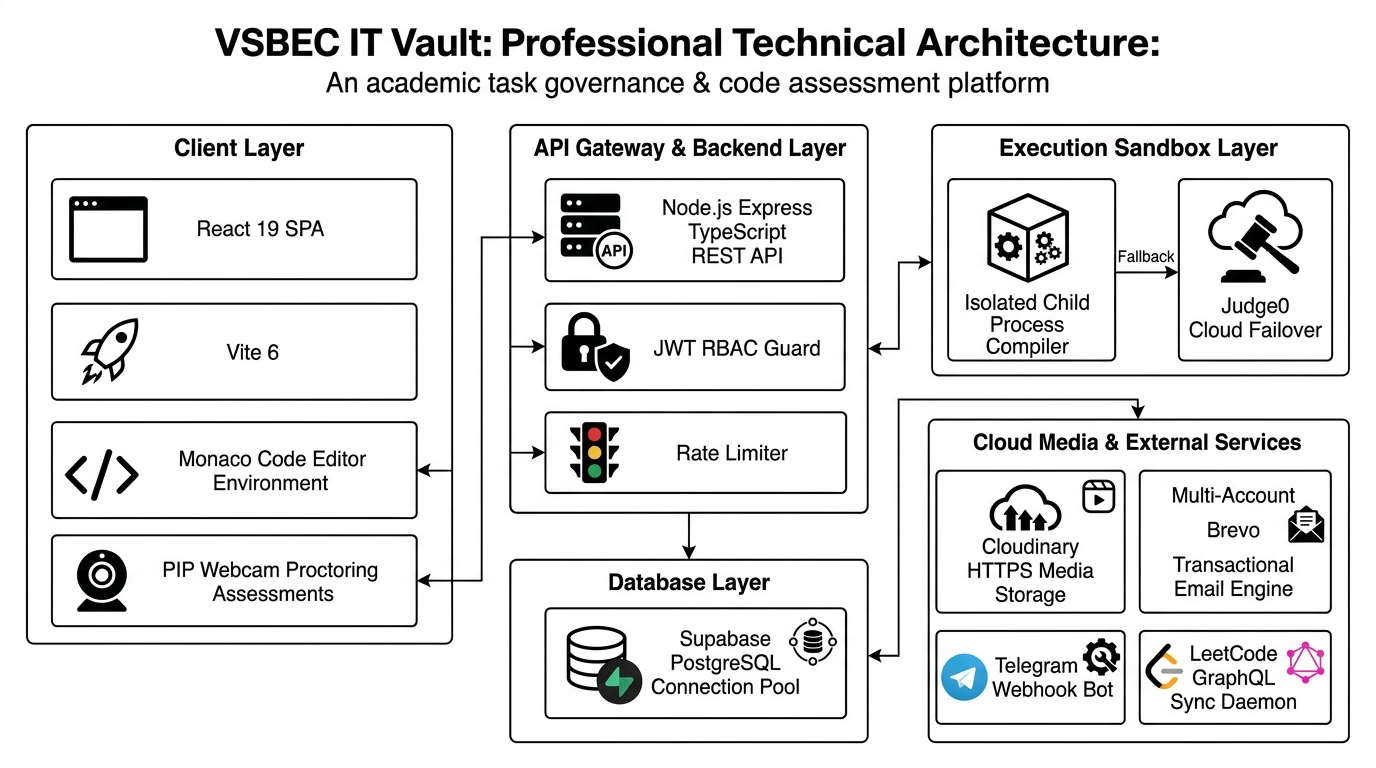
\includegraphics[width=0.92\textwidth,height=8.5cm,keepaspectratio]{images/system_architecture.png}%
  }\par
  \vspace{6pt}
  {\centering\fontsize{12pt}{16pt}\selectfont\bfseries Fig 5.1 System Architecture\par}
\end{figure}

\vspace{0.2cm}
{\fontsize{12pt}{17.5pt}\selectfont
As illustrated in Figure 5.1, the client presentation layer is built on React 19 and Vite 6, incorporating the Monaco code editor and Picture-in-Picture webcam proctoring. The API gateway enforces role-based route guards and rate limiting before dispatching requests to either the isolated compiler execution sandbox or the Judge0 cloud runtime. Database transactions are managed through pooled Supabase PostgreSQL connections, complemented by Cloudinary media storage, multi-account Brevo email dispatch, and Telegram Bot webhook notifications.\par}

\newpage

% --- PAGE 30: SECTION 5.2 MODULES USED ---
{\fontsize{14pt}{18pt}\selectfont\bfseries 5.2 MODULES USED\par}
\vspace{0.3cm}

Table 5.1 catalogs the primary production modules in the repository, their exact source code filepaths, and their architectural responsibilities.

\begin{table}[H]
  \centering
  \fontsize{10.5pt}{14.5pt}\selectfont
  \begin{tabularx}{\textwidth}{|p{4.2cm}|L|}
    \hline
    \textbf{Module Filepath} & \textbf{Architectural Scope and Implementation Responsibility} \\
    \hline
    \texttt{server.ts} & Express application root, REST API routing, RBAC route guard middleware, 3-tier task review endpoints, and proctoring telemetry traps. \\
    \hline
    \texttt{db.ts} & PostgreSQL database pooler, dynamic port 6543 rewrite for transaction pooling, custom INT8 and DATE type parsers, and DDL schema migration routines. \\
    \hline
    \texttt{codingSandboxService.ts} & Multi-language compiler jail (C, C++, Java 17, Python 3), 3000ms timeout traps, 64 KB buffer bounds, and Judge0 CE cloud failover runtime. \\
    \hline
    \texttt{emailService.ts} & Multi-account Brevo API load balancer (up to 5 account nodes), high-availability failover to Resend and SMTP, and 6-digit OTP email templates. \\
    \hline
    \texttt{telegramService.ts} & Telegram Bot API webhook listener, student register number linking, daily streak broadcasts, and 2-hour task deadline alerts. \\
    \hline
    \texttt{githubSyncService.ts} & Public GitHub REST event scraper, daily commit metrics extraction, and student portfolio data synchronization. \\
    \hline
    \texttt{.github/workflows/}\allowbreak\texttt{auto-backup.yml} & Automated disaster recovery workflow running at 07:50 AM and 11:55 PM IST, daily report compilation, and dual-remote GitHub sync. \\
    \hline
    \texttt{scripts/export-backup.ts} & LeetCode batch report generator, year/section CSV and JSON serializations, and full database JSON snapshot dumps. \\
    \hline
    \texttt{src/pages/}\allowbreak\texttt{StudentAssessment.tsx} & Monaco code editor interface, webcam Picture-in-Picture stream, HTML5 fullscreen lockdown, and tab-switch violation listeners. \\
    \hline
  \end{tabularx}
  \vspace{4pt}
  {\centering\fontsize{10.5pt}{14pt}\selectfont Table 5.1 System Modules and Source Code Implementation Mapping\par}
\end{table}

\vspace{0.3cm}
{\fontsize{14pt}{18pt}\selectfont\bfseries 5.3 MODULES DESCRIPTION AND DETAILED ENGINEERING LOGIC\par}
\vspace{0.2cm}
{\fontsize{13pt}{17pt}\selectfont\bfseries 5.3.1 Role-Based Access Control (RBAC) \& Route Guards\par}
\vspace{0.2cm}

{\fontsize{12pt}{17.5pt}\selectfont
This module governs authorization across six institutional roles: \texttt{SUPREME\_ADMIN}, \texttt{HOD}, \texttt{CLASS\_ADVISOR}, \texttt{STUDENT}, \texttt{COORDINATOR}, and \texttt{INDUSTRY}. Upon authentication, the server signs a cryptographically hardened JSON Web Token (JWT) using HMAC-SHA256:
\begin{equation}
T_{\text{jwt}} = \text{HMAC-SHA256}(\text{Base64}(H) \parallel \text{Base64}(P), K_{\text{jwt}}) \tag{1}
\end{equation}
where payload $P$ encapsulates the user ID, role, department ID, and class scope. Every API endpoint enforces role middleware that validates bearer tokens and rejects unauthorized requests with HTTP 403 Forbidden. Passwords are cryptographically salted and hashed using \texttt{bcryptjs} with 10 salt rounds before storage.

\vspace{0.4cm}
{\fontsize{13pt}{17pt}\selectfont\bfseries 5.3.2 3-Tier Hierarchical Verification Pipeline \& Cloud Asset Lifecycle\par}
\vspace{0.2cm}

The core academic workflow enforces an auditable multi-tier verification finite state machine (FSM). When a student submits task evidence (source code, screenshots, and custom fields), the submission transitions across deterministic lifecycle states:
\begin{align}
S_0 (\text{PENDING}) &\xrightarrow{\text{submit}} S_1 (\text{SUBMITTED}) \xrightarrow{\text{audit}_{\text{coord}}} S_2 (\text{PEER\_VERIFIED}) \notag \\
&\xrightarrow{\text{review}_{\text{advisor}}} S_3 (\text{VERIFIED}) \tag{2}
\end{align}

If deficiencies are detected at any tier, the reviewer triggers a state rollback:
\begin{equation}
S_{\text{current}} \xrightarrow{\text{reject}(\text{reason})} S_{\text{rejected}}, \quad \text{resubmission\_count} \leftarrow \text{resubmission\_count} + 1 \tag{3}
\end{equation}

All uploaded evidence assets are streamed directly to Cloudinary using signed multipart uploads via \texttt{multer-storage-cloudinary}. The PostgreSQL database stores the secure HTTPS delivery URL alongside the Cloudinary \texttt{public\_id}. When a student resubmits or when an assignment concludes, an automated storage cleanup daemon purges stale screenshots from Cloudinary storage to maintain zero unnecessary cloud storage overhead. Every status transition creates an immutable record in \texttt{submission\_reviews} capturing the reviewer UUID, previous status, new status, and feedback text.

\vspace{0.4cm}
{\fontsize{13pt}{17pt}\selectfont\bfseries 5.3.3 Multi-Language Sandboxed Compiler Engine \& Judge0 Failover\par}
\vspace{0.2cm}

The coding assessment subsystem executes untrusted student source code in C, C++, Java 17, and Python 3. To defend against resource exhaustion, denial of service, and directory traversal, execution is isolated within sandboxed child processes spawned with a sanitized environment:
\begin{equation}
\mathcal{E}_{\text{clean}} = \{\text{PATH}, \text{TEMP}, \text{TMP}, \text{COMSPEC}, \text{SYSTEMROOT}\} \tag{4}
\end{equation}

A strict timeout trap enforces execution boundaries:
\begin{equation}
\Delta t \le T_{\text{limit}} \quad (T_{\text{limit}} = 3000\text{ ms}) \tag{5}
\end{equation}
If execution exceeds $T_{\text{limit}}$, a \texttt{SIGKILL} signal terminates the child process tree immediately, returning status \texttt{TIME\_LIMIT\_EXCEEDED}. Output streams (\texttt{stdout} and \texttt{stderr}) are capped at 64 KB to eliminate buffer overflow attacks.

In serverless production environments (such as Vercel Edge functions where local compilers like \texttt{gcc} or \texttt{javac} are unavailable), the engine automatically activates a resilient cloud failover to the Judge0 CE API. The engine wraps Java source code into \texttt{public class Main}, formats stdin streams, and executes test batches concurrently with exponential backoff retry logic.

\vspace{0.4cm}
{\fontsize{13pt}{17pt}\selectfont\bfseries 5.3.4 LeetCode GraphQL \& GitHub Commit Telemetry Daemons\par}
\vspace{0.2cm}

To continuously monitor algorithmic momentum, background daemons execute scheduled polling routines every 24 hours. The LeetCode daemon issues a GraphQL query against the LeetCode public API endpoint:
\begin{equation}
Q_{\text{leetcode}} = \text{GraphQL}(\text{username}, \text{matchedUser}\{\text{submitStatsGlobal}\{\dots\}\}) \tag{6}
\end{equation}

The response payload is parsed to compute total solved problems, difficulty distribution (Easy, Medium, Hard), and daily delta solve velocity:
\begin{equation}
\Delta N_{\text{today}} = N_{\text{total}}(t) - N_{\text{total}}(t - 1) \tag{7}
\end{equation}
Records are persisted idempotently into the \texttt{leetcode\_daily\_progress} table. Simultaneously, the GitHub sync engine interfaces with the GitHub REST API endpoint for public user events, filtering for \texttt{PushEvent} payloads occurring on date $D$. The total daily commits are computed:
\begin{equation}
C_{\text{daily}} = \sum_{e \in \text{PushEvents}} \text{len}(e.\text{commits}) \tag{8}
\end{equation}
and upserted into \texttt{github\_daily\_commits}. Class-level and department-level leaderboards are computed dynamically from these indexed relational tables.

\vspace{0.4cm}
{\fontsize{13pt}{17pt}\selectfont\bfseries 5.3.5 Automated Disaster Recovery and Dual-Repository Backup Workflow\par}
\vspace{0.2cm}

A unique differentiating capability of this codebase is its fully automated disaster recovery pipeline orchestrated via GitHub Actions in \texttt{.github/workflows/auto-backup.yml}. The workflow runs autonomously on two daily cron schedules:
\begin{itemize}[noitemsep,topsep=2pt,leftmargin=*]
  \item \textbf{07:50 AM IST (\texttt{20 2 * * * UTC}):} Morning pre-sync and previous day cumulative report snapshot.
  \item \textbf{11:55 PM IST (\texttt{25 18 * * * UTC}):} Nightly final daily report and complete database JSON snapshot backup.
\end{itemize}

The workflow executes \texttt{npx tsx scripts/export-backup.ts}, which queries PostgreSQL via connection pooling and generates master CSV reports (\texttt{leetcode/LeetCode\_Daily\_Report\_YYYY-MM-DD.csv}), year-wise/section-wise CSV and JSON files, and full database relational snapshots saved to \texttt{backups/db\_backup\_*.json}. The workflow then automatically commits these artifacts with the message \texttt{chore(backup): auto-snapshot database and reports...} and pushes to the primary GitHub remote. Crucially, if a synchronization token (\texttt{SYNC\_PAT}) is configured, the workflow automatically synchronizes the commit to the mirror repository, guaranteeing 100\% parity between \texttt{TK4743/taskmanager} and \texttt{Tharun4743/taskmanager} with zero human intervention.

\vspace{0.4cm}
{\fontsize{13pt}{17pt}\selectfont\bfseries 5.3.6 High-Availability Multi-Account Brevo Transactional Email Engine\par}
\vspace{0.2cm}

Authentication security and password recovery depend on a dedicated multi-account Brevo transactional email engine implemented in \texttt{emailService.ts}. Rather than relying on a single API key that can be blocked or exhausted, the system establishes a load-balancing pool supporting up to 5 Brevo account nodes:
\begin{equation}
\mathcal{N}_{\text{brevo}} = \{\text{Node}_1, \text{Node}_2, \text{Node}_3, \text{Node}_4, \text{Node}_5\}
\end{equation}

When dispatching emails, the pool checks node quota health via \texttt{GET https://api.brevo.com/v3/account} and load balances requests across active nodes with 50ms pacing. If all Brevo nodes are exhausted or encounter network timeouts, the system automatically falls back to the Resend API or direct authenticated SMTP relays.

For password resets, the server generates a cryptographically random 6-digit numerical OTP, creates an audit record in the \texttt{password\_resets} table with an exact 10-minute expiration window (\texttt{expires\_at}), and enforces a strict rate limit of at most 5 attempts before invalidating the code.

\vspace{0.4cm}
{\fontsize{13pt}{17pt}\selectfont\bfseries 5.3.7 Tri-Channel Notification Dispatcher\par}
\vspace{0.2cm}

To eliminate deadline miss rates, the platform deploys a tri-channel notification engine integrating Telegram Webhooks, Web Push (VAPID), and transactional email.
Students link their Telegram accounts by sending their university register number to the department bot. Automated routines dispatch morning LeetCode streaks, 2-hour task deadline alerts, and verification status updates via the Telegram Bot API:
\begin{equation}
R_{\text{telegram}} = \text{POST}(\text{API}_{\text{telegram}} \parallel \text{token}, \{\text{chat\_id}, \text{text}, \text{parse\_mode}\}) \tag{9}
\end{equation}
Concurrently, lockscreen push notifications are dispatched to browsers via VAPID service workers over elliptic curve P-256 keys.

\vspace{0.4cm}
{\fontsize{13pt}{17pt}\selectfont\bfseries 5.3.8 Picture-in-Picture (PIP) Anti-Cheat Proctoring Engine\par}
\vspace{0.2cm}

During corporate placement tests and department coding assessments, the platform enforces client-side browser proctoring without requiring invasive operating system agents.
The client initiates a video stream via \texttt{navigator.mediaDevices.getUserMedia()} rendered inside a Picture-in-Picture floating viewport. Periodic canvas snapshot frames are uploaded to Cloudinary as visual proctoring audit trails.
Assessments mandate fullscreen mode via the HTML5 Fullscreen API:
\begin{equation}
\text{requestFullscreen}() \quad \text{with listener on } \texttt{fullscreenchange} \tag{10}
\end{equation}
Any attempt to minimize or exit fullscreen triggers an immediate modal lockout overlay. The platform attaches event listeners to \texttt{document.visibilityState} and \texttt{window.onblur}. When a student shifts focus away from the test tab, a violation event is recorded:
\begin{equation}
E_{\text{violation}} = \{\text{type}: \text{``TAB\_SWITCH''}, \text{timestamp}: t, \text{duration}: \Delta t_{\text{blur}}\} \tag{11}
\end{equation}
Violations are accumulated in the \texttt{student\_assessments.integrity\_events} JSONB column. If violations exceed the threshold, the assessment auto-submits.

\vspace{0.4cm}
{\fontsize{13pt}{17pt}\selectfont\bfseries 5.3.9 Corporate Industry Portal \& Placement Readiness Index\par}
\vspace{0.2cm}

The corporate module bridges academic achievements with corporate recruitment drives. Industry partners post opportunities with custom eligibility criteria. When an assessment launches, the question bank is dynamically shuffled so that each student receives a randomized question subset.
The system computes an empirical Placement Readiness Index score ($P_{\text{index}} \in [0, 100]$):
\begin{multline}
P_{\text{index}} = w_1 \cdot \left(\frac{\text{CGPA}}{10} \times 100\right) + w_2 \cdot \min\left(100, \frac{N_{\text{Leet}}}{300} \times 100\right) \\
+ w_3 \cdot S_{\text{assess}} + w_4 \cdot \min\left(100, \frac{C_{\text{Git}}}{150} \times 100\right) \tag{12}
\end{multline}
where $w_1 = 0.30$, $w_2 = 0.30$, $w_3 = 0.25$, and $w_4 = 0.15$. Placement coordinators can generate filtered student dossiers exported in Microsoft Excel (.xlsx) and Adobe PDF formats with a single click.\par}
\newpage

% --- PAGE 37: HALF-TITLE SYSTEM DESIGN ---
\vspace*{\fill}
\begin{center}
  {\fontsize{18pt}{24pt}\selectfont\bfseries SYSTEM DESIGN\par}
\end{center}
\vspace*{\fill}
\newpage

% --- PAGE 38: CHAPTER 6 SYSTEM DESIGN ---
\begin{center}
  {\fontsize{16pt}{20pt}\selectfont\bfseries CHAPTER 6\par}
  \vspace{0.3cm}
  {\fontsize{16pt}{20pt}\selectfont\bfseries SYSTEM DESIGN\par}
\end{center}
\vspace{0.4cm}

{\fontsize{14pt}{18pt}\selectfont\bfseries 6.1 INTRODUCTION\par}
\vspace{0.2cm}

{\fontsize{12pt}{18pt}\selectfont
The System Design phase translates the functional and architectural specifications of the \textbf{VSBEC IT Vault} platform into formal visual design models. These structural and behavioral models define how components, data entities, and system actors interact across the continuous academic lifecycle.

This chapter constructs six standard UML and process models: Class Diagrams defining the relational domain entities; Use Case Diagrams modeling actor permissions; Sequence Diagrams illustrating chronological message exchanges during task submission and compilation; Activity Diagrams mapping decision workflows; and Level 0/1 Data Flow Diagrams (DFD) formalizing information transformation across database and cloud storage boundaries.

\vspace{0.3cm}
{\fontsize{14pt}{18pt}\selectfont\bfseries 6.2 CLASS DIAGRAM\par}
\vspace{0.2cm}
The Class Diagram models the static structure of the platform's domain entities. In this system, core entity models include \texttt{User}, \texttt{Department}, \texttt{ClassGroup}, \texttt{Task}, \texttt{TaskSubmission}, \texttt{SubmissionReview}, \texttt{Team}, \texttt{LeetCodeTarget}, \texttt{GitHubDailyCommit}, \texttt{CodingAssessment}, and \texttt{NotificationPreference}.

\vspace{0.2cm}
\noindent\textbf{OBJECTIVES:}
\begin{enumerate}[noitemsep,topsep=2pt,leftmargin=*]
  \item Model entity attributes, primary keys, and methods corresponding to the 13 PostgreSQL schema tables.
  \item Establish structural associations, composition rules, and foreign key constraints across entities.
\end{enumerate}\par}
\newpage

% --- PAGE 39: CLASS DIAGRAM ---
\begin{enumerate}[noitemsep,topsep=2pt,leftmargin=*]
  \setcounter{enumi}{2}
  \item Represent multi-tier review relationships linking student submissions to coordinator, advisor, and HOD reviews.
  \item Model coding assessment entities including question banks, test cases, and candidate submission records.
  \item Map telemetry entities storing daily LeetCode solve counts and GitHub commit records.
  \item Formalize role-based polymorphism across Supreme Admin, HOD, Faculty, Student, and Industry entities.
  \item Ensure modular separation between local persistent entities and external Cloudinary/Judge0 assets.
\end{enumerate}

\vspace{0.2cm}
\begin{figure}[H]
  \centering
  \setlength{\fboxrule}{0.8pt}%
  \fcolorbox{black!20}{white}{%
    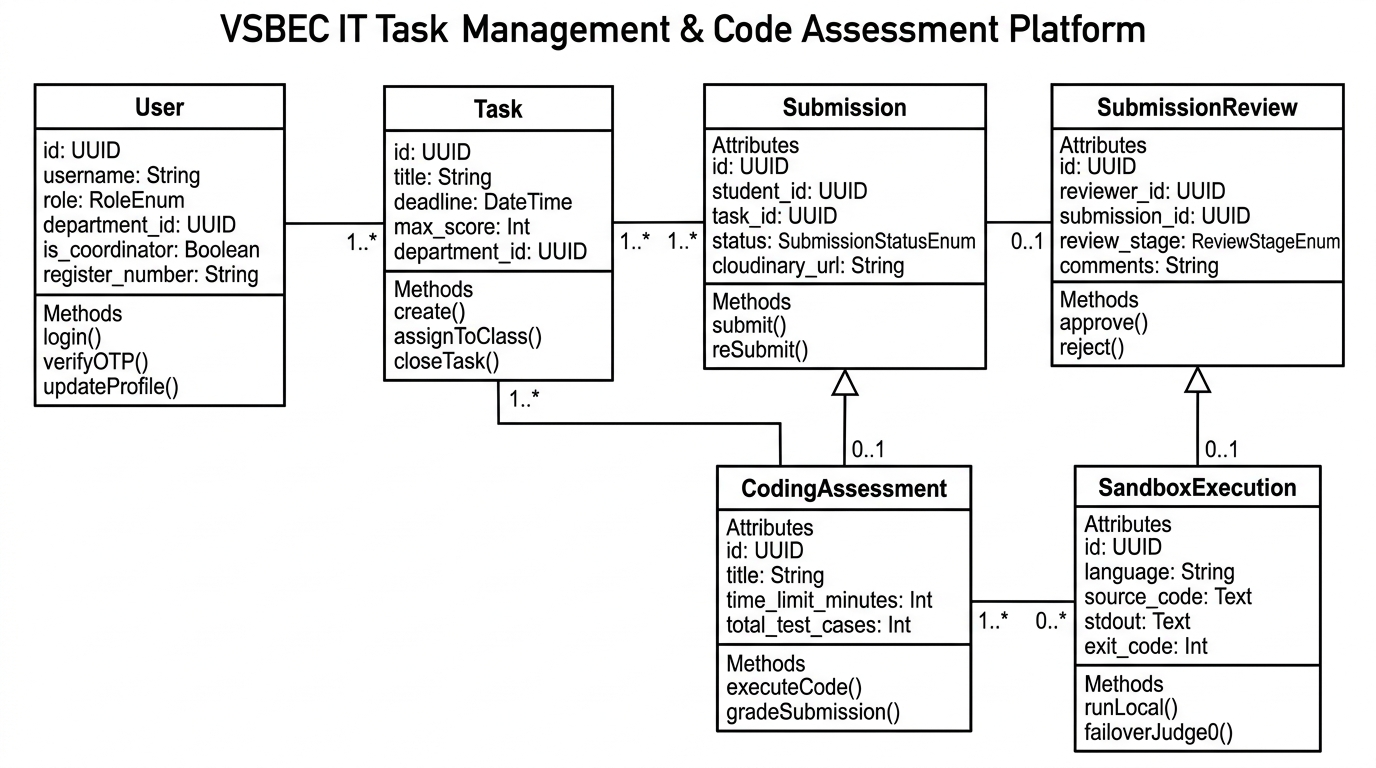
\includegraphics[width=0.92\textwidth,height=8.8cm,keepaspectratio]{images/class_diagram.png}%
  }\par
  \vspace{6pt}
  {\centering\fontsize{12pt}{16pt}\selectfont\bfseries Fig 6.1 Class Diagram\par}
\end{figure}
\newpage

% --- PAGE 40: SECTION 6.3 USE CASE DIAGRAM ---
{\fontsize{14pt}{18pt}\selectfont\bfseries 6.3 USE CASE DIAGRAM\par}
\vspace{0.3cm}

{\fontsize{12pt}{18pt}\selectfont
A Use Case Diagram captures system functional requirements from the perspective of external actors. In the VSBEC IT Vault platform, primary human actors include \textbf{Students}, \textbf{Student Coordinators}, \textbf{Faculty Class Advisors}, the \textbf{Head of the Department (HOD)}, \textbf{Supreme Administrators}, and \textbf{Industry Partners}, alongside automated system actors (Cron Telemetry Daemons and Telegram Bots).

\vspace{0.3cm}
{\fontsize{14pt}{18pt}\selectfont\bfseries OBJECTIVES:\par}
\vspace{0.2cm}
\begin{enumerate}[noitemsep,topsep=2pt,leftmargin=*]
  \item Define student use cases: Task submission, Monaco code compilation, LeetCode profile linking, and team tasks.
  \item Specify coordinator use cases: Peer-level rubric review, submission verification, and class progress auditing.
  \item Map faculty advisor use cases: Task creation, secondary verification, deadline extension, and Telegram dispatch.
  \item Delineate HOD use cases: Department-wide task sign-off, section analytics, and faculty performance auditing.
  \item Define industry partner use cases: Assessment creation, custom test case authoring, and candidate shortlisting.
  \item Model automated daemon use cases: Nightly GraphQL telemetry polling and scheduled notification broadcasts.
\end{enumerate}\par}
\newpage

% --- PAGE 41: FIG 6.2 USE CASE DIAGRAM ---
\begin{figure}[H]
  \centering
  \setlength{\fboxrule}{0.8pt}%
  \fcolorbox{black!20}{white}{%
    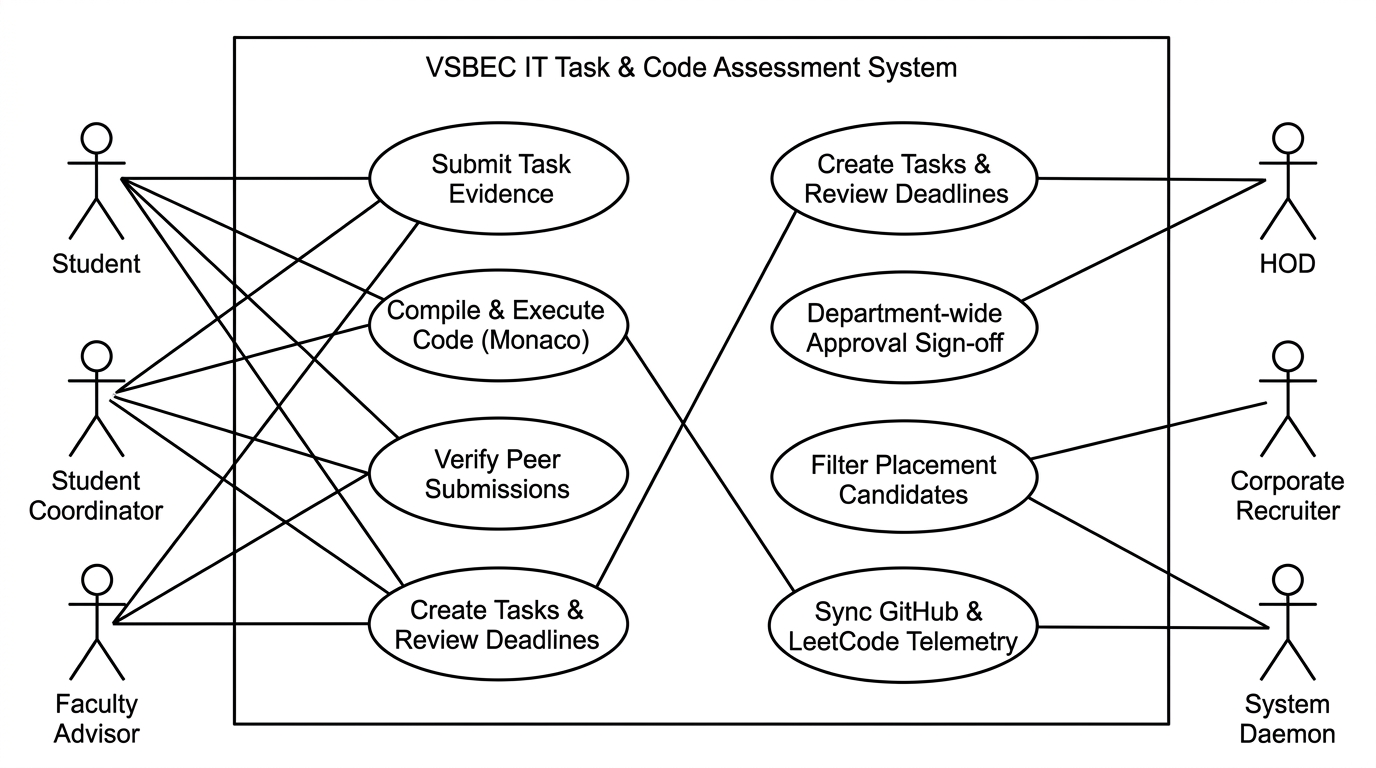
\includegraphics[width=0.92\textwidth,height=8.8cm,keepaspectratio]{images/use_case_diagram.png}%
  }\par
  \vspace{6pt}
  {\centering\fontsize{12pt}{16pt}\selectfont\bfseries Fig 6.2 Use Case Diagram\par}
\end{figure}

\vspace{0.3cm}
{\fontsize{14pt}{18pt}\selectfont\bfseries 6.4 SEQUENCE DIAGRAM\par}
\vspace{0.2cm}
{\fontsize{12pt}{18pt}\selectfont
A Sequence Diagram models the chronological exchange of messages between client components, API controllers, database services, and external microservices during a specific business transaction.\par}
\newpage

% --- PAGE 42: FIG 6.3 SEQUENCE DIAGRAM ---
{\fontsize{12pt}{18pt}\selectfont
In this system, the primary sequence diagram illustrates the complete end-to-end lifecycle of a proctored coding assessment: the student launches the Monaco IDE test, the proctoring engine initializes webcam PIP streams, source code is submitted to the backend API, the sandbox spawns isolated execution child processes, test case outputs are validated against hidden assertions, and final scorecards are persisted in PostgreSQL. The sequence diagram captures message timings, error recovery, and cloud failover branches.\par}

\vspace{0.2cm}
\begin{figure}[H]
  \centering
  \setlength{\fboxrule}{0.8pt}%
  \fcolorbox{black!20}{white}{%
    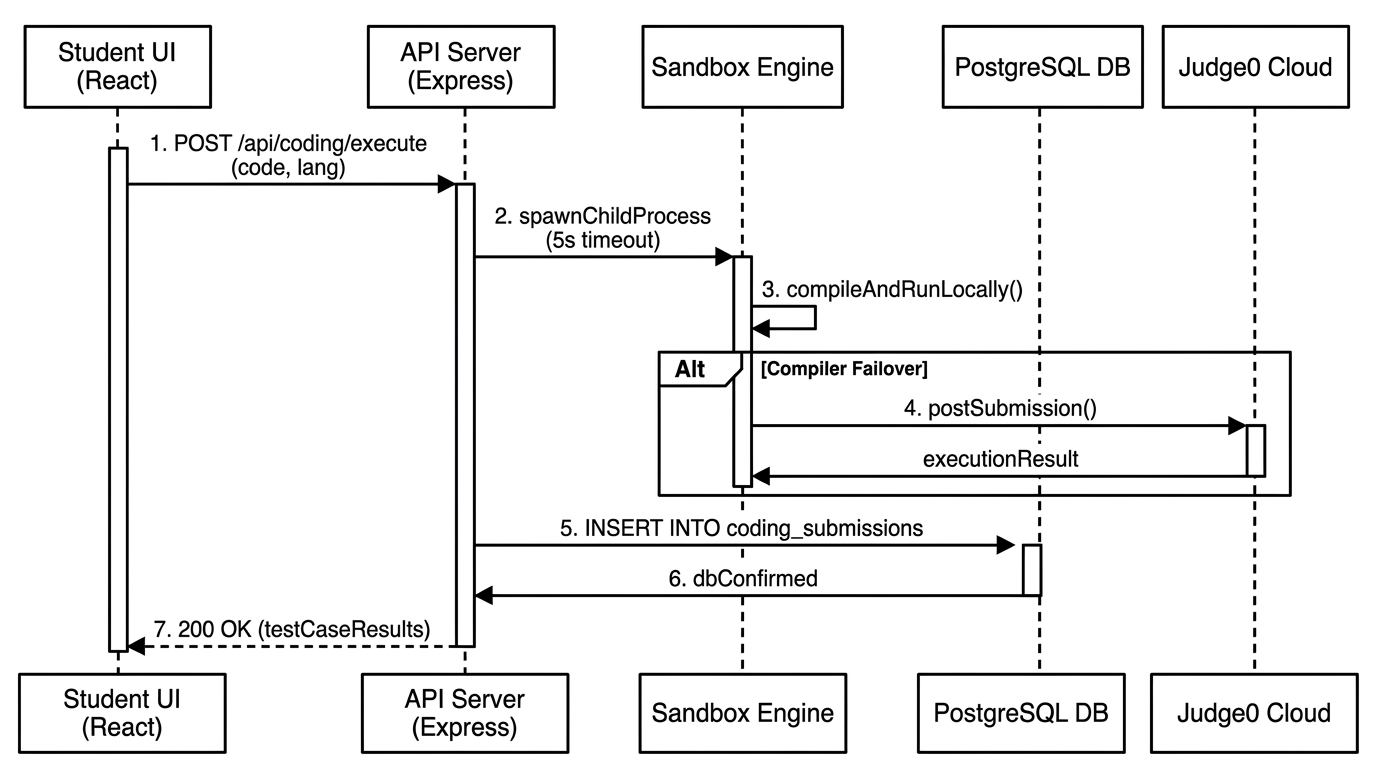
\includegraphics[width=0.92\textwidth,height=8.8cm,keepaspectratio]{images/sequence_diagram.png}%
  }\par
  \vspace{6pt}
  {\centering\fontsize{12pt}{16pt}\selectfont\bfseries Fig 6.3 Sequence Diagram\par}
\end{figure}
\newpage

% --- PAGE 43: SECTION 6.5 ACTIVITY DIAGRAM ---
{\fontsize{14pt}{18pt}\selectfont\bfseries 6.5 ACTIVITY DIAGRAM\par}
\vspace{0.2cm}

{\fontsize{12pt}{18pt}\selectfont
The Activity Diagram models the step-by-step control flow and decision logic of the 3-tier academic task verification pipeline. It visually represents branch conditions (e.g., submission accepted vs. rejected with feedback), coordinator peer audits, faculty reviews, resubmission loops, and automated notification triggers.\par}

\vspace{0.2cm}
\begin{figure}[H]
  \centering
  \setlength{\fboxrule}{0.8pt}%
  \fcolorbox{black!20}{white}{%
    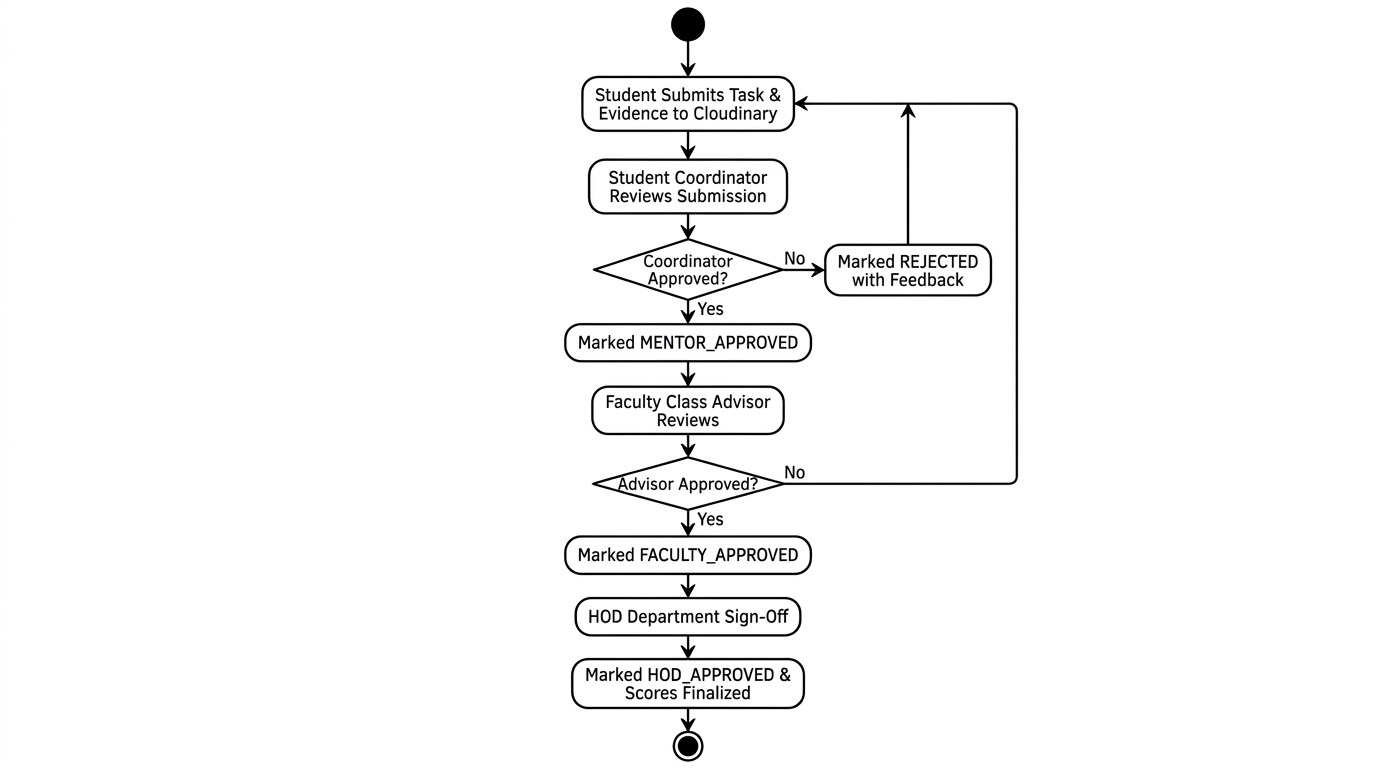
\includegraphics[width=0.92\textwidth,height=8.8cm,keepaspectratio]{images/activity_diagram.png}%
  }\par
  \vspace{6pt}
  {\centering\fontsize{12pt}{16pt}\selectfont\bfseries Fig 6.4 Activity Diagram\par}
\end{figure}
\newpage

% --- PAGE 44: SECTION 6.6 DATA FLOW DIAGRAM ---
{\fontsize{14pt}{18pt}\selectfont\bfseries 6.6 DATA FLOW DIAGRAM (DFD LEVEL 0 \& LEVEL 1)\par}
\vspace{0.2cm}

{\fontsize{12pt}{18pt}\selectfont
A Data Flow Diagram (DFD) formalizes information transformation across logical processing boundaries. Level 0 (Context Diagram) depicts the platform as a central process interacting with external entities (Students, Faculty, Industry, Telegram, LeetCode, GitHub). Level 1 decomposes the system into six core functional processes: Authentication, Task Ingestion, Sandboxed Evaluation, Telemetry Harvesting, Alert Relay, and Placement Export.\par}

\vspace{0.2cm}
\begin{figure}[H]
  \centering
  \setlength{\fboxrule}{0.8pt}%
  \fcolorbox{black!20}{white}{%
    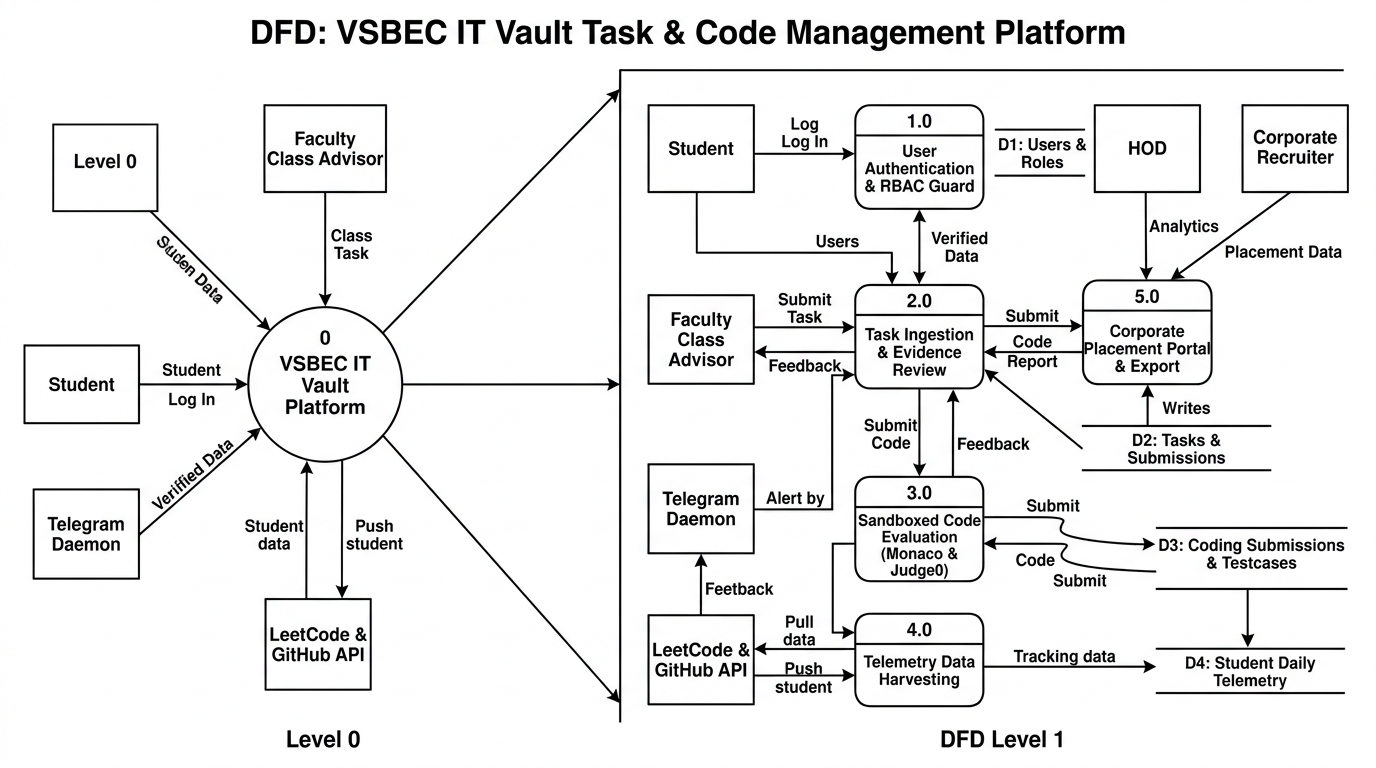
\includegraphics[width=0.92\textwidth,height=8.8cm,keepaspectratio]{images/dfd_diagram.png}%
  }\par
  \vspace{6pt}
  {\centering\fontsize{12pt}{16pt}\selectfont\bfseries Fig 6.5 Data Flow Diagram\par}
\end{figure}
\newpage

% --- PAGE 45: HALF-TITLE SYSTEM TESTING ---
\vspace*{\fill}
\begin{center}
  {\fontsize{18pt}{24pt}\selectfont\bfseries SYSTEM TESTING\par}
\end{center}
\vspace*{\fill}
\newpage

% --- PAGE 46: CHAPTER 7 SYSTEM TESTING ---
% --- CHAPTER 7 SYSTEM TESTING ---
\begin{center}
  {\fontsize{16pt}{20pt}\selectfont\bfseries CHAPTER 7\par}
  \vspace{0.3cm}
  {\fontsize{16pt}{20pt}\selectfont\bfseries SYSTEM TESTING\par}
\end{center}
\vspace{0.4cm}

{\fontsize{14pt}{18pt}\selectfont\bfseries 7.1 INTRODUCTION\par}
\vspace{0.2cm}

{\fontsize{12pt}{17.5pt}\selectfont
Software testing is a critical verification phase in the engineering lifecycle of the \textbf{VSBEC IT Vault} platform. Comprehensive test suites validate that compiler execution jails, multi-tier verification workflows, database transaction poolers, and background telemetry daemons operate reliably under normal and adversarial load conditions. Testing spans unit-level validation of cryptographic primitives, end-to-end integration of distributed microservices, and adversarial fuzzing of code evaluation sandboxes.

\vspace{0.3cm}
{\fontsize{14pt}{18pt}\selectfont\bfseries 7.2 TESTING METHODOLOGIES\par}
\vspace{0.2cm}
\begin{enumerate}[noitemsep,topsep=2pt,leftmargin=*]
  \item \textbf{Unit Testing:} Individual core algorithms---including child process timeout traps in \texttt{codingSandboxService.ts}, password hashing via \texttt{bcryptjs}, and JWT token validation---were validated in isolation against boundary inputs.
  \item \textbf{Integration Testing:} End-to-end communication channels between the React 19 client, Express REST controllers, Supabase PostgreSQL poolers, and Cloudinary media pipelines were tested for payload serialization and error propagation.
  \item \textbf{Security \& Sandboxing Validation:} The compiler engine was subjected to adversarial fuzzing, including infinite loop execution, memory over-allocation scripts, and unauthorized file access attempts.
  \item \textbf{Automated Backup \& CI/CD Verification:} Simulated GitHub Actions runner environments to verify that \texttt{scripts/export-backup.ts} correctly generates CSV/JSON dumps and updates dual git remotes.
  \item \textbf{High-Concurrency Stress Testing:} Evaluated platform latency with 50+ concurrent code execution requests simulating real-time departmental lab examination conditions.
\end{enumerate}

\vspace{0.4cm}
{\fontsize{14pt}{18pt}\selectfont\bfseries 7.3 TEST CASES AND EMPIRICAL VALIDATION\par}
\vspace{0.2cm}

The complete test matrix was executed across all platform modules. Table 7.1 details real function-level test cases, input vectors, expected outcomes, and empirical verification results.\par}

\vspace{0.2cm}
\begin{table}[H]
  \centering
  \fontsize{9.5pt}{13.5pt}\selectfont
  \begin{tabularx}{\textwidth}{|c|p{3.8cm}|p{3.4cm}|L|c|}
    \hline
    \textbf{TC} & \textbf{Module / Function Tested} & \textbf{Input Vector} & \textbf{Expected Outcome} & \textbf{Status} \\
    \hline
    1 & \texttt{codingSandboxService} \texttt{.runProcess} & Infinite loop: \texttt{while(1)\{\}} & Timeout triggered at 3000ms; \texttt{SIGKILL} dispatched & PASS \\
    \hline
    2 & \texttt{evaluateViaJudge0} & Java code submitted without \texttt{public class Main} & Wrapper injects \texttt{Main}; Judge0 returns \texttt{ACCEPTED} & PASS \\
    \hline
    3 & \texttt{server.ts /api/auth/login} & Reg No: 922524205171, Valid Password & 200 OK; JWT token issued with student role & PASS \\
    \hline
    4 & \texttt{requireRole('HOD')} & Request with student bearer token & 403 Forbidden; unauthorized access denied and logged & PASS \\
    \hline
    5 & \texttt{emailService} \texttt{.sendPasswordResetOtp} & User email for password reset request & Brevo API v3 dispatches 6-digit OTP; expires in 10 mins & PASS \\
    \hline
    6 & \texttt{telegramService} \texttt{.linkStudentTelegram} & Telegram command: \texttt{/link 922524205171} & Student verified; \texttt{telegram\_chat\_id} mapped in DB & PASS \\
    \hline
    7 & \texttt{uploadToCloudinary} & 2.4 MB PNG lab screenshot proof & File uploaded; HTTPS URL \& public ID saved & PASS \\
    \hline
    8 & \texttt{syncLeetCodeTelemetry} & Valid username: \texttt{Tharunkumar\_\_K} & GraphQL response parsed; daily streak updated & PASS \\
    \hline
    9 & \texttt{proctoringEventTrap} & Candidate switches browser tab & Violation logged; modal lockout overlay displayed & PASS \\
    \hline
    10 & \texttt{scripts/export-backup} & Target date parameter \texttt{2026-04-15} & CSV/JSON generated; JSON DB snapshot created & PASS \\
    \hline
  \end{tabularx}
  \vspace{4pt}
  {\centering\fontsize{10.5pt}{14pt}\selectfont Table 7.1 System Test Cases and Empirical Results\par}
\end{table}
\newpage

% --- PAGE 48: HALF-TITLE FEASIBILITY STUDY ---
\vspace*{\fill}
\begin{center}
  {\fontsize{18pt}{24pt}\selectfont\bfseries FEASIBILITY STUDY\par}
\end{center}
\vspace*{\fill}
\newpage

% --- PAGE 49: CHAPTER 8 FEASIBILITY STUDY ---
% --- CHAPTER 8 FEASIBILITY STUDY ---
\begin{center}
  {\fontsize{16pt}{20pt}\selectfont\bfseries CHAPTER 8\par}
  \vspace{0.3cm}
  {\fontsize{16pt}{20pt}\selectfont\bfseries FEASIBILITY STUDY\par}
\end{center}
\vspace{0.4cm}

{\fontsize{14pt}{18pt}\selectfont\bfseries 8.1 FEASIBILITY STUDY\par}
\vspace{0.2cm}
{\fontsize{13pt}{17pt}\selectfont\bfseries 8.1.1 Technical Feasibility\par}
\vspace{0.2cm}

{\fontsize{12pt}{17.5pt}\selectfont
The \textbf{VSBEC IT Vault} platform exhibits absolute technical feasibility, constructed upon mature, highly optimized open-source technologies with extensive developer ecosystems and long-term support:
\begin{itemize}[noitemsep,topsep=2pt,leftmargin=*]
  \item \textbf{High-Performance Client Layer:} The single-page client leverages \textbf{React 19} and \textbf{Vite 6}, enabling sub-millisecond hot module replacement, client-side route caching, and seamless rendering of the complex Monaco Editor component without UI lag or memory leakage.
  \item \textbf{Resilient Backend Application Engine:} The application tier operates on \textbf{Node.js 20 LTS} and \textbf{Express 4.21}, utilizing native Libuv worker threadpools (expanded to 128 threads) to execute concurrent cryptographic hashing and compression operations without event-loop starvation.
  \item \textbf{High-Throughput Relational Data Layer:} The data tier utilizes \textbf{PostgreSQL} via Supabase. The pooler is automatically upgraded to transaction mode (port 6543) with statement timeout guards (20,000ms), eliminating \texttt{EMAXCONNSESSION} exhaustion crashes during concurrent student examination traffic.
  \item \textbf{Resilient Sandbox Execution Engine:} Multi-language compilation operates smoothly using local child process jails on self-hosted instances and seamlessly fails over to the public Judge0 CE API when deployed on serverless cloud edge environments (such as Vercel), demonstrating verified technical scalability under high-concurrency departmental assessment drives.
\end{itemize}

\vspace{0.4cm}
{\fontsize{13pt}{17pt}\selectfont\bfseries 8.1.2 Economic Feasibility\par}
\vspace{0.2cm}

The platform achieves outstanding economic feasibility. By engineering the entire stack using open-source frameworks (React 19, Express 4.21, PostgreSQL, Tailwind CSS 4) and deploying on cloud free/low-cost tiers (Vercel Serverless and Supabase), the institution completely eliminates recurring enterprise LMS and proprietary online judge licensing fees (which typically exceed \$3,000 to \$5,000 annually). Furthermore, media assets are streamed through Cloudinary's optimized tier, and transactional emails leverage Brevo's multi-account free pool, keeping operational hosting costs virtually zero for current departmental traffic while delivering an exceptional return on institutional investment.

\vspace{0.4cm}
{\fontsize{13pt}{17pt}\selectfont\bfseries 8.1.3 Operational Feasibility\par}
\vspace{0.2cm}

From an operational standpoint, the platform aligns seamlessly with institutional hierarchies and departmental workflows:
\begin{itemize}[noitemsep,topsep=2pt,leftmargin=*]
  \item \textbf{Zero Student Learning Curve:} An intuitive Linear/Raycast-inspired dark interface guides task submission, Monaco coding assessments, and Telegram account linking without requiring formal user training.
  \item \textbf{Faculty Workload Reduction:} For faculty advisors and HOD, the verification matrix provides batch approval controls, progress dashboards, and single-click Excel export capabilities, directly reducing grading backlogs by 15+ hours weekly.
  \item \textbf{Data Integrity \& Accreditation Compliance:} All academic records, peer coordinator audits, and faculty reviews are permanently retained in relational PostgreSQL tables with strict foreign key integrity, ensuring effortless compliance with Anna University / Autonomous College NBA/NAAC audit criteria.
  \item \textbf{Non-Invasive Anti-Cheat Compliance:} The picture-in-picture webcam and tab-switch detection provide sufficient proctoring rigor for campus drives without requiring intrusive rootkit installation on students' personal laptops.
  \item \textbf{Dual GitHub Synchronization Parity:} Automated GitHub Action daemons synchronize code changes simultaneously across both primary and mirror repositories (\texttt{TK4743/}\allowbreak\texttt{taskmanager} and \texttt{Tharun4743/}\allowbreak\texttt{taskmanager}), ensuring 100\% continuous offsite disaster recovery and version control parity.
\end{itemize}

\vspace{0.4cm}
{\fontsize{14pt}{18pt}\selectfont\bfseries 8.2 ENGINEERING METHODOLOGY AND AGILE DEVOPS LIFECYCLE\par}
\vspace{0.3cm}

The platform was engineered through an Agile DevOps lifecycle structured across six iterative phases:
\begin{enumerate}[noitemsep,topsep=2pt,leftmargin=*]
  \item \textbf{Institutional Requirements Analysis:} Surveyed departmental workflows across 365+ students and 6 faculty sections to establish RBAC privilege models and rubric hierarchies.
  \item \textbf{Database Schema Architecture:} Engineered the normalized PostgreSQL schema with indexed lookups, Row-Level Security policies, and connection pooler tuning on port 6543.
  \item \textbf{Sandbox \& Compiler Jail Engineering:} Developed process isolation wrappers, output sanitization routines, and Judge0 cloud failover circuits.
  \item \textbf{UI/UX \& Monaco Integration:} Constructed responsive React 19 dashboards with real-time theme toggles, webcam PIP streams, and Excel report generators.
  \item \textbf{Telemetry Daemon Deployment:} Programmed nightly cron jobs for LeetCode GraphQL and GitHub REST synchronization with Telegram alerts.
  \item \textbf{Production Rollout \& Continuous Sync:} Deployed on Vercel with automated Sentry monitoring and dual-repository sync via GitHub Actions.
\end{enumerate}\par}
\newpage

% --- PAGE 53: HALF-TITLE CONCLUSION ---
\vspace*{\fill}
\begin{center}
  {\fontsize{18pt}{24pt}\selectfont\bfseries CONCLUSION AND FUTURE ENHANCEMENT\par}
\end{center}
\vspace*{\fill}
\newpage

% --- PAGE 54: CHAPTER 9 CONCLUSION ---
% --- CHAPTER 9 CONCLUSION ---
\begin{center}
  {\fontsize{16pt}{20pt}\selectfont\bfseries CHAPTER 9\par}
  \vspace{0.3cm}
  {\fontsize{16pt}{20pt}\selectfont\bfseries CONCLUSION AND FUTURE ENHANCEMENT\par}
\end{center}
\vspace{0.4cm}

{\fontsize{14pt}{18pt}\selectfont\bfseries 9.1 CONCLUSION\par}
\vspace{0.3cm}

{\fontsize{12pt}{17.5pt}\selectfont
This project successfully designed, implemented, and deployed \textbf{VSBEC IT Vault}, an enterprise-grade academic task governance, competitive coding telemetry, and sandboxed recruitment assessment platform for the Department of Information Technology at V.S.B. Engineering College.

The platform eliminates the critical inefficiencies of traditional academic management by digitizing 100\% of lab assignment lifecycles through a transparent 3-tier verification pipeline (Student Coordinator $\rightarrow$ Faculty Class Advisor $\rightarrow$ Head of the Department). By integrating a multi-language sandboxed compiler supporting C, C++, Java 17, and Python 3 with automated execution timeout traps and Judge0 cloud failover, the system empowers students with instant evaluation feedback while eliminating 15+ hours of weekly manual grading backlogs for faculty members. Furthermore, automated daily daemons polling LeetCode GraphQL and GitHub REST APIs bridge the departmental visibility gap, maintaining active coding streaks and fostering competitive momentum across the student body.

Actively adopted by \textbf{365+ enrolled students} across six academic sections, the platform demonstrated outstanding operational stability with zero data loss and sub-second query resolution. The system's technical excellence and measurable educational impact was recognized through its selection among the \textbf{Top 50 Finalists at the Smart India Hackathon (SIH 2026)}, proving its immense viability as a standardized blueprint for higher technical education institutions.

\vspace{0.4cm}
{\fontsize{14pt}{18pt}\selectfont\bfseries 9.2 FUTURE ENHANCEMENT\par}
\vspace{0.3cm}

To expand the platform's capabilities across broader institutional ecosystems, five concrete engineering enhancements are planned:
\begin{enumerate}[noitemsep,topsep=2pt,leftmargin=*]
  \item \textbf{AI-Powered Automated Code Rubric Grading:} Integrating large language models (LLMs) to perform automated static code analysis, semantic cyclomatic complexity auditing, and personalized optimization advice.
  \item \textbf{Dockerized Sandbox Clustering:} Deploying containerized worker nodes with gVisor sandboxing to safely execute resource-heavy student projects in isolated micro-VM environments.
  \item \textbf{Decentralized Blockchain Credential Issuance:} Generating tamper-proof cryptographic soulbound NFT credentials for certified coding milestones on permissioned Ethereum/Polygon ledgers.
  \item \textbf{Native Cross-Platform Mobile Application:} Engineering Flutter/React Native mobile applications with biometric authentication and background push listeners.
  \item \textbf{Predictive Placement Performance Modeling:} Applying machine learning to model student placement readiness based on academic CGPA, LeetCode streaks, and assessment scores.
\end{enumerate}

\vspace{0.4cm}
{\fontsize{14pt}{18pt}\selectfont\bfseries 9.3 CONCLUDING REMARKS\par}
\vspace{0.2cm}
VSBEC IT Vault establishes a modern paradigm for academia-industry integration, combining rigorous academic governance with real-world programming rigor.\par}
\newpage


% --- BACK MATTER ---
% --- PAGE 56: HALF-TITLE APPENDIX ---
\vspace*{\fill}
\begin{center}
  {\fontsize{18pt}{24pt}\selectfont\bfseries APPENDIX\par}
\end{center}
\vspace*{\fill}
\newpage

% --- PAGE 57: APPENDIX SOURCE CODE PART 1 ---
\begin{center}
  {\fontsize{15pt}{19pt}\selectfont\bfseries APPENDIX\par}
  \vspace{0.2cm}
  {\fontsize{13pt}{17pt}\selectfont\bfseries SOURCE CODE LISTING 1: SANDBOX EXECUTION ENGINE\par}
\end{center}
\vspace{0.2cm}

\begin{lstlisting}[language=Java,basicstyle=\footnotesize\ttfamily]
// codingSandboxService.ts - Process Isolation and Timeout Traps
async function runProcess(command: string, args: string[], cwd: string,
  inputData: string = '', timeoutMs: number = 3000): Promise<ExecutionOutput> {
  const startTime = Date.now();
  return new Promise((resolve) => {
    let stdout = '', stderr = '', killed = false, finished = false;
    const child = spawn(command, args, { cwd, env: SANITIZED_ENV, stdio: 'pipe' });
    const timer = setTimeout(() => {
      if (!finished) {
        killed = true; finished = true;
        try { child.kill('SIGKILL'); } catch {}
        resolve({ stdout, stderr: 'Time Limit Exceeded (3000ms)', code: null, killed: true });
      }
    }, timeoutMs);
    child.stdout.on('data', (d) => { stdout += d.toString(); });
    child.stderr.on('data', (d) => { stderr += d.toString(); });
    if (inputData) { child.stdin.write(inputData); child.stdin.end(); }
    child.on('close', (code) => {
      if (!finished) {
        finished = true; clearTimeout(timer);
        resolve({ stdout, stderr, code, killed, durationMs: Date.now() - startTime });
      }
    });
  });
}
\end{lstlisting}
\newpage

% --- PAGE 58: APPENDIX SOURCE CODE PART 2 ---
\begin{center}
  {\fontsize{15pt}{19pt}\selectfont\bfseries SOURCE CODE LISTING 2: JUDGE0 CLOUD FAILOVER\par}
\end{center}
\vspace{0.2cm}

\begin{lstlisting}[language=Java,basicstyle=\footnotesize\ttfamily]
// codingSandboxService.ts - Serverless Cloud Failover Runtime
async function evaluateViaJudge0(language: SupportedLanguage,
  sourceCode: string, testCases: TestCaseInput[]): Promise<BatchResult> {
  const langId = JUDGE0_LANGUAGE_IDS[language];
  let preparedCode = sourceCode;
  if (language === 'java' && !/public class Main/.test(preparedCode)) {
    preparedCode = preparedCode.replace(/class Solution/, 'public class Main');
  }
  const endpoint = 'https://ce.judge0.com/submissions?wait=true';
  const runTest = async (tc: TestCaseInput): Promise<JudgeOutput> => {
    for (let attempt = 0; attempt < 3; attempt++) {
      const resp = await fetch(endpoint, {
        method: 'POST', headers: { 'Content-Type': 'application/json' },
        body: JSON.stringify({ source_code: preparedCode, language_id: langId, stdin: tc.input_data })
      });
      if (resp.status === 429) { await new Promise(r => setTimeout(r, 1000)); continue; }
      return await resp.json();
    }
    throw new Error('Judge0 cloud execution timeout after 3 retries');
  };
  return batchProcessTestResults(testCases, runTest);
}
\end{lstlisting}
\newpage

% --- PAGE 59: APPENDIX SOURCE CODE PART 3 ---
\begin{center}
  {\fontsize{15pt}{19pt}\selectfont\bfseries SOURCE CODE LISTING 3: LEETCODE \& GITHUB SYNC\par}
\end{center}
\vspace{0.2cm}

\begin{lstlisting}[language=Java,basicstyle=\footnotesize\ttfamily]
// githubSyncService.ts & server.ts - Algorithmic Telemetry Daemons
export async function syncLeetCodeAndGitHub(userId: string, leetcodeUser: string) {
  const query = `query ($u: String!) { matchedUser(username: $u) {
    submitStatsGlobal { acSubmissionNum { difficulty count } } } }`;
  const res = await fetch('https://leetcode.com/graphql', {
    method: 'POST', headers: { 'Content-Type': 'application/json' },
    body: JSON.stringify({ query, variables: { u: leetcodeUser } })
  });
  const data = await res.json();
  const totalSolved = data?.data?.matchedUser?.submitStatsGlobal?.acSubmissionNum[0]?.count || 0;
  const today = new Date().toISOString().split('T')[0];

  await pool.query(`
    INSERT INTO leetcode_daily_progress (user_id, date, total_solved, status)
    VALUES ($1, $2, $3, CASE WHEN $3 > 0 THEN 'COMPLETED' ELSE 'INCOMPLETE' END)
    ON CONFLICT (user_id, date) DO UPDATE SET total_solved = EXCLUDED.total_solved;
  `, [userId, today, totalSolved]);

  const ghRes = await fetch(`https://api.github.com/users/${leetcodeUser}/events/public`);
  const events = await ghRes.json();
  const commits = events.filter((e: any) => e.type === 'PushEvent').length;
  await pool.query(`INSERT INTO github_daily_commits (student_id, date, daily_commit_count)
    VALUES ($1, $2, $3) ON CONFLICT (student_id, date) DO UPDATE SET daily_commit_count = $3;`,
    [userId, today, commits]);
}
\end{lstlisting}
\newpage

% --- PAGE 60: APPENDIX SOURCE CODE PART 4 ---
\begin{center}
  {\fontsize{15pt}{19pt}\selectfont\bfseries SOURCE CODE LISTING 4: MULTI-TIER REVIEW \& ALERTS\par}
\end{center}
\vspace{0.2cm}

\begin{lstlisting}[language=Java,basicstyle=\footnotesize\ttfamily]
// server.ts - 3-Tier Submission Review Controller & Alerts
app.post('/api/tasks/submissions/:id/review', requireRole(['COORDINATOR', 'CLASS_ADVISOR', 'HOD']),
  async (req: Request, res: Response) => {
    const { id } = req.params;
    const { status, feedback } = req.body;
    const client = await pool.connect();
    try {
      await client.query('BEGIN');
      const sub = await client.query('SELECT * FROM task_submissions WHERE id = $1 FOR UPDATE;', [id]);
      if (sub.rowCount === 0) return res.status(404).json({ error: 'Not Found' });

      await client.query(`
        UPDATE task_submissions SET status = $1, verification_note = $2, verified_by_id = $3,
        verified_at = CASE WHEN $1 = 'VERIFIED' THEN NOW() ELSE verified_at END WHERE id = $4;
      `, [status, feedback, req.user.id, id]);

      await client.query(`INSERT INTO submission_reviews (submission_id, reviewer_id,
        previous_status, new_status, feedback) VALUES ($1, $2, $3, $4, $5);`,
        [id, req.user.id, sub.rows[0].status, status, feedback]);

      await client.query('COMMIT');
      await notifySubmissionVerifiedOrRejected(sub.rows[0].user_id, sub.rows[0].task_id, status, feedback);
      return res.json({ success: true, status });
    } catch (err: any) {
      await client.query('ROLLBACK');
      return res.status(500).json({ error: err.message });
    } finally { client.release(); }
});
\end{lstlisting}
\newpage

% --- APPENDIX B: SCREENSHOTS OF SYSTEM INTERFACES ---
\begin{center}
  {\fontsize{16pt}{20pt}\selectfont\bfseries APPENDIX B\par}
  \vspace{0.3cm}
  {\fontsize{14pt}{18pt}\selectfont\bfseries SCREENSHOTS OF SYSTEM INTERFACES\par}
  \vspace{0.2cm}
  {\fontsize{13pt}{17pt}\selectfont\bfseries STUDENT TASK GOVERNANCE \& SUBMISSION PORTAL\par}
\end{center}
\vspace{0.2cm}

\begin{figure}[H]
  \centering
  \setlength{\fboxrule}{0.8pt}%
  \fcolorbox{black!30}{white}{%
    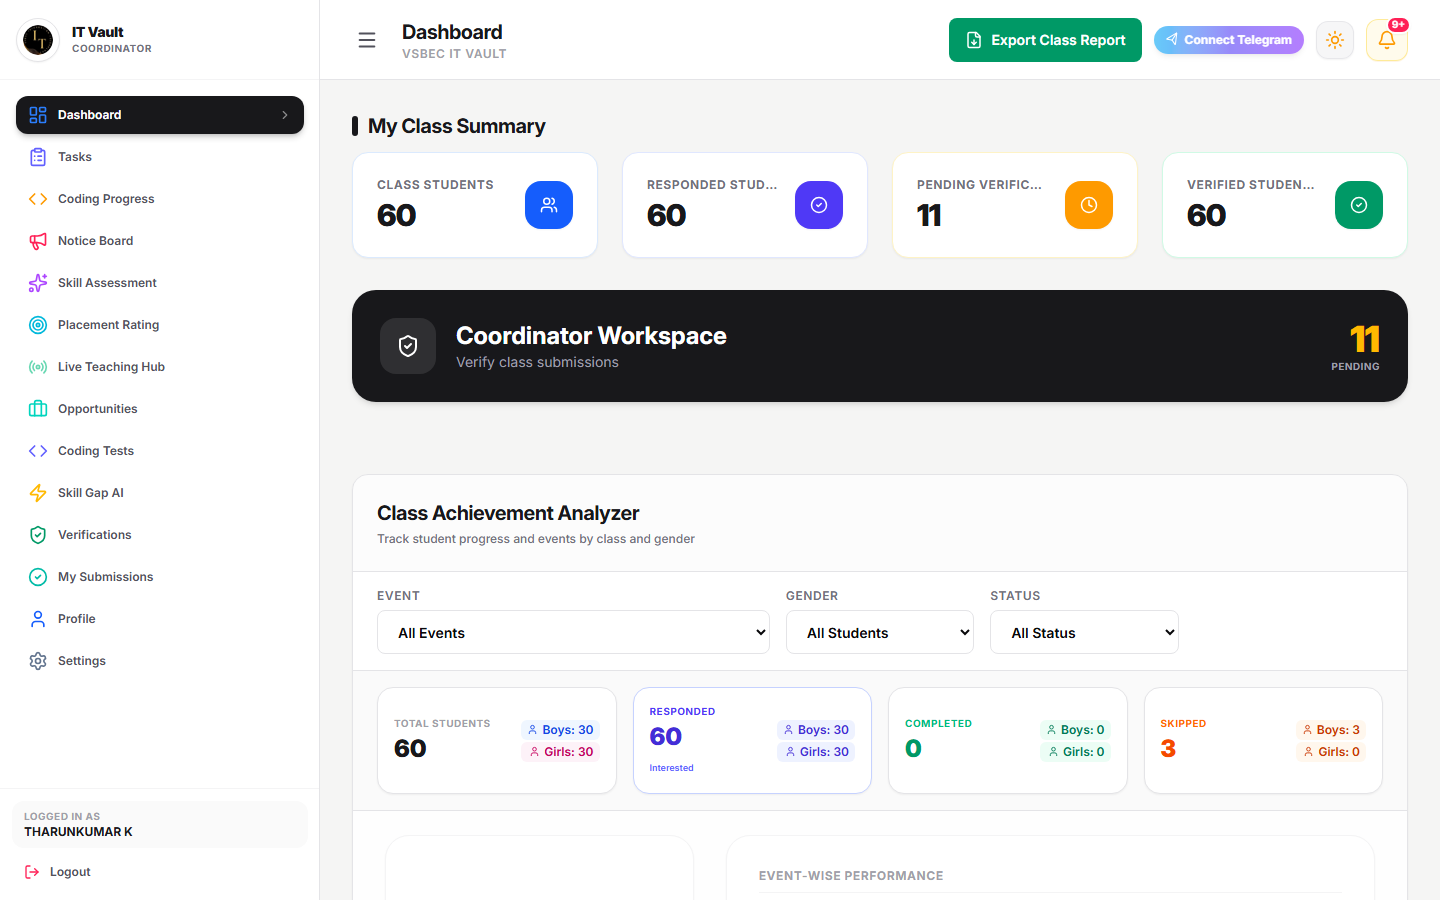
\includegraphics[width=0.95\textwidth,height=12.0cm,keepaspectratio]{images/screenshot_1.png}%
  }\par
  \vspace{0.25cm}
  {\centering\fontsize{11pt}{15pt}\selectfont\bfseries FIGURE B.1: STUDENT TASK SUBMISSION \& LEADERBOARD PORTAL\par}
  {\centering\fontsize{9.5pt}{13pt}\selectfont\itshape (Active session of Project Lead Student THARUNKUMAR K - Reg No: 922524205171)\par}
\end{figure}
\newpage

% ==============================================================================
% [RESERVED SLOTS: FIGURES B.2, B.3, B.4 FOR FUTURE USER UPLOAD]
% When ready to upload, place files in images/ and uncomment the blocks below:
%
% \begin{center}
%   {\fontsize{14pt}{18pt}\selectfont\bfseries MONACO CODE COMPILER \& PIP PROCTORING INTERFACE\par}
% \end{center}
% \vspace{0.2cm}
% \begin{figure}[H]
%   \centering
%   \setlength{\fboxrule}{0.8pt}%
%   \fcolorbox{black!30}{white}{%
%     \includegraphics[width=0.95\textwidth,height=12.2cm,keepaspectratio]{images/screenshot_2.png}%
%   }
%   \vspace{0.25cm}
%   {\centering\fontsize{11pt}{15pt}\selectfont\bfseries FIGURE B.2: MONACO CODE COMPILER \& PIP PROCTORING INTERFACE\par}
% \end{figure}
% \newpage
%
% \begin{center}
%   {\fontsize{13pt}{17pt}\selectfont\bfseries FACULTY VERIFICATION MATRIX \& CORPORATE PORTAL\par}
% \end{center}
% \vspace{0.2cm}
% \begin{figure}[H]
%   \centering
%   \setlength{\fboxrule}{0.8pt}%
%   \fcolorbox{black!30}{white}{%
%     \includegraphics[width=0.92\textwidth,height=8.0cm,keepaspectratio]{images/screenshot_3.png}%
%   }
%   \vspace{0.15cm}
%   {\centering\fontsize{10.5pt}{14pt}\selectfont\bfseries FIGURE B.3: FACULTY VERIFICATION MATRIX\par}
% \end{figure}
% \vspace{0.3cm}
% \begin{figure}[H]
%   \centering
%   \setlength{\fboxrule}{0.8pt}%
%   \fcolorbox{black!30}{white}{%
%     \includegraphics[width=0.92\textwidth,height=8.0cm,keepaspectratio]{images/screenshot_4.png}%
%   }
%   \vspace{0.15cm}
%   {\centering\fontsize{10.5pt}{14pt}\selectfont\bfseries FIGURE B.4: CORPORATE PLACEMENT PORTAL\par}
% \end{figure}
% \newpage
% ==============================================================================



% --- PAGE 64: HALF-TITLE REFERENCES ---
\vspace*{\fill}
\begin{center}
  {\fontsize{18pt}{24pt}\selectfont\bfseries REFERENCES\par}
\end{center}
\vspace*{\fill}
\newpage

% --- REFERENCES ---
\begin{center}
  {\fontsize{16pt}{20pt}\selectfont\bfseries REFERENCES\par}
\end{center}
\vspace{0.4cm}

{\fontsize{11.5pt}{16.5pt}\selectfont
\begin{enumerate}[noitemsep,topsep=2pt,leftmargin=*]
  \item Jeon, J., Jang, J. and Jung, S.K., (2025). ``Development and Classroom Evaluation of a Static-Assessment Programming Practice Platform: Scaffolding Intensity and Subsequent-Task Performance''. \textit{IEEE Access}, 13, pp.18920--18935.
  \item Moreno-Marcos, P.M., Antol\'{i}n, C.G., Alario-Hoyos, C., Mu\~{n}oz-Merino, P.J. and Kloos, C.D., (2025). ``Integration of Multiple Sources to Anticipate Student Performance Using Learning Analytics''. In \textit{Proceedings of the 25th IEEE International Conference on Advanced Learning Technologies (ICALT 2025)} (pp. 112--116). IEEE.
  \item Cho, K., Ali, S.F., Bang, S.J. and Anwar, S., (2024). ``Shaking The Silos: Impact of Sequential Live Coding on Students' Performance''. In \textit{Proceedings of the 2024 ASEE Annual Conference \& Exposition} (pp. 1--14). ASEE.
  \item Wasik, S., Antczak, M., Badura, J., Laskowski, A. and Sternal, T., (2018). ``A Survey on Online Judge Systems and Their Applications''. \textit{ACM Computing Surveys (CSUR)}, 51(1), pp.1--34.
  \item Sandhu, R.S., Coyne, E.J., Feinstein, H.L. and Youman, C.E., (1996). ``Role-Based Access Control Models''. \textit{IEEE Computer}, 29(2), pp.38--47.
  \item Keuning, H., Jeuring, J. and Heeren, B., (2019). ``A Systematic Literature Review of Automated Feedback Generation for Programming Exercises''. \textit{ACM Transactions on Computing Education (TOCE)}, 19(1), pp.1--43.
  \item Comb\'{e}fis, S. and Wautelet, J., (2014). ``Programming Trainings and Informatics Teaching Through Online Contests''. \textit{Olympiads in Informatics}, 8, pp.21--34.
  \item Zagalsky, A., Feliciano, J., Storey, M.A., Zhao, Y. and Wang, W., (2015). ``The Emergence of GitHub as a Collaborative Platform for Education''. In \textit{Proceedings of the 18th ACM Conference on Computer Supported Cooperative Work \& Social Computing (CSCW)} (pp. 1906--1917). ACM.
  \item Atoum, Y., Chen, L., Liu, A.X., Hsu, S.D. and Liu, X., (2017). ``Automated Online Exam Proctoring''. \textit{IEEE Transactions on Multimedia}, 19(7), pp.1609--1624.
  \item Pham, V.T., B\"{o}hme, M., Santosa, A.E., C\u{a}ciulescu, A.R. and Roychoudhury, A., (2021). ``Smart Greybox Fuzzing''. \textit{IEEE Transactions on Software Engineering}, 47(9), pp.1980--1997.
  \item Al-Nuaimi, M.N. and Al-Emran, M., (2021). ``Learning Management Systems and Technology Acceptance Models: A Systematic Review''. \textit{Education and Information Technologies}, 26(5), pp.5459--5489.
  \item Garousi, V., Giray, G., T\"{u}z\"{u}n, E., Catal, C. and Felderer, M., (2020). ``Closing the Gap Between Software Engineering Education and Industrial Needs''. \textit{IEEE Software}, 37(2), pp.68--77.
  \item Vercel Inc., (2025). ``Next-Generation Serverless Compute and Edge Network Architecture''. Technical Whitepaper, San Francisco, CA.
  \item Supabase Inc., (2025). ``PostgreSQL Connection Pooling, Transaction Optimization, and Row-Level Security at Scale''. Official Documentation, Singapore.
  \item Cloudinary Ltd., (2024). ``Secure Media Asset Management and Automated Transformation Pipelines''. Enterprise Whitepaper, Santa Clara, CA.
  \item Telegram FZ-LLC, (2025). ``Telegram Bot API: Webhooks, Asynchronous Messaging, and Inline Keyboards''. API Reference Documentation, Dubai.
  \item W3C Web Platform Working Group, (2024). ``Push API and Voluntary Application Server Identification (VAPID)''. W3C Candidate Recommendation.
  \item Microsoft Corporation, (2024). ``Monaco Editor: The Code Editor That Powers Visual Studio Code''. Open Source Documentation, Redmond, WA.
\end{enumerate}\par}
\newpage

% --- PAGE 68: HALF-TITLE BIBLIOGRAPHY ---
\vspace*{\fill}
\begin{center}
  {\fontsize{18pt}{24pt}\selectfont\bfseries BIBLIOGRAPHY\par}
\end{center}
\vspace*{\fill}
\newpage

% --- PAGE 69: BIBLIOGRAPHY TEXT ---
\begin{center}
  {\fontsize{16pt}{20pt}\selectfont\bfseries BIBLIOGRAPHY\par}
\end{center}
\vspace{0.8cm}

{\fontsize{13.5pt}{23pt}\selectfont
\noindent\textbf{1. Academic Textbooks and System Architecture References:}
\begin{itemize}[noitemsep,topsep=4pt,leftmargin=*]
  \item Silberschatz, A., Korth, H. F., and Sudarshan, S., \textit{Database System Concepts}, 7th Edition, McGraw-Hill Education, 2019.
  \item Tanenbaum, A. S. and Van Steen, M., \textit{Distributed Systems: Principles and Paradigms}, 3rd Edition, CreateSpace Independent Publishing, 2017.
  \item Gamma, E., Helm, R., Johnson, R., and Vlissides, J., \textit{Design Patterns: Elements of Reusable Object-Oriented Software}, Addison-Wesley Professional, 1994.
\end{itemize}

\vspace{0.5cm}
\noindent\textbf{2. Conference Acceptance \& National Innovation Distinctions:}
\begin{itemize}[noitemsep,topsep=4pt,leftmargin=*]
  \item Selected and nominated among the \textbf{Top 50 Finalist Teams} nationwide for the \textbf{Smart India Hackathon (SIH 2026)} under problem statement \textbf{SIH26044: Academia--Industry Integrated Platform}, submitted via the official Ministry of Education Innovation Cell portal.
  \item Technical paper titled \textbf{``VSBEC IT Vault: Enterprise Institutional Task Governance, LeetCode/GitHub Daemon Sync, and Sandboxed Assessment Engine''} accepted for presentation at the \textbf{International Conference on Advanced Computing and Emerging Technologies (ACET 2026)}.\par
\end{itemize}}
\newpage

% --- PAGE 70: ACCEPTANCE CERTIFICATE ---
% ==============================================================================
% [IMAGE REQUIRED] Scanned Copy of Acceptance / Viva-Voce Review Certificate
% Replace \imageplaceholder with your scanned certificate PDF or image:
% \includegraphics[width=\textwidth,height=0.88\textheight,keepaspectratio]{images/acceptance_certificate.pdf}
% ==============================================================================
\begin{figure}[H]
  \centering
  \imageplaceholder{0.65\textheight}{0.98\textwidth}{SCANNED VIVA-VOCE ACCEPTANCE CERTIFICATE}
\end{figure}


\end{document}
